\part{C++ Basics}
\chapter{C++}
\section{C++ }
\textbf{Formål:} Dette afsnit introducerer grundlæggende C++-begreber, som er essentielle for at programmere Arduino. Studerende vil lære om syntaks, output, kommentarer, variabler, brugerinput, datatyper, operatorer, strings, betingelser og loops. Disse emner danner grundlaget for at forstå mere avancerede koncepter og anvende dem i Arduino-projekter.
\newline\newline
\noindent\textbf{Læringsmål:} Efter at have læst dette afsnit forventes det, at studerende kan:
\begin{itemize}
	\item Forstå og skrive grundlæggende C++-syntaks.
	\item Udføre input og output operationer med Arduino.
	\item Bruge kommentarer til at dokumentere Arduino-kode.
	\item Deklarere og anvende variabler i Arduino-programmer.
	\item Modtage brugerinput fra Arduino-sensorer og behandle det.
	\item Identificere og anvende forskellige datatyper i Arduino-programmer.
	\item Anvende operatorer til forskellige operationer på Arduino.
	\item Håndtere strings effektivt i Arduino-kode.
	\item Skrive og forstå betingede udsagn (if-else) i Arduino-programmer.
	\item Implementere loops (while og for) for gentagne opgaver på Arduino.
\end{itemize}

\section{C++ Syntax}
\textbf{Teori:} C++ syntaks refererer til de regler og strukturer, der definerer hvordan man skriver et gyldigt C++ program. I Arduino IDE skrives C++ kode for at styre mikrocontrollerens funktioner. Et typisk Arduino-program består af to centrale funktioner:
\begin{itemize}
	\item \textbf{\texttt{setup()}}: Kører én gang, når Arduino'en starter. Bruges til initialisering.
	\item \textbf{\texttt{loop()}}: Kører kontinuerligt, efter \texttt{setup()} er udført. Bruges til hovedlogikken.
\end{itemize}
Disse funktioner definerer programflowet og strukturen i et Arduino-program.
\newline\newline
\noindent\textbf{Eksempel:}
\begin{lstlisting}[language=C++]
	void setup() {
		// initial setup code
		pinMode(13, OUTPUT); // Set pin 13 as output
	}
	
	void loop() {
		// repeated execution code
		digitalWrite(13, HIGH); // Turn on the LED
		delay(1000); // Wait for 1 second
		digitalWrite(13, LOW); // Turn off the LED
		delay(1000); // Wait for 1 second
	}
\end{lstlisting}
\begin{figure}[h!]
	\centering
	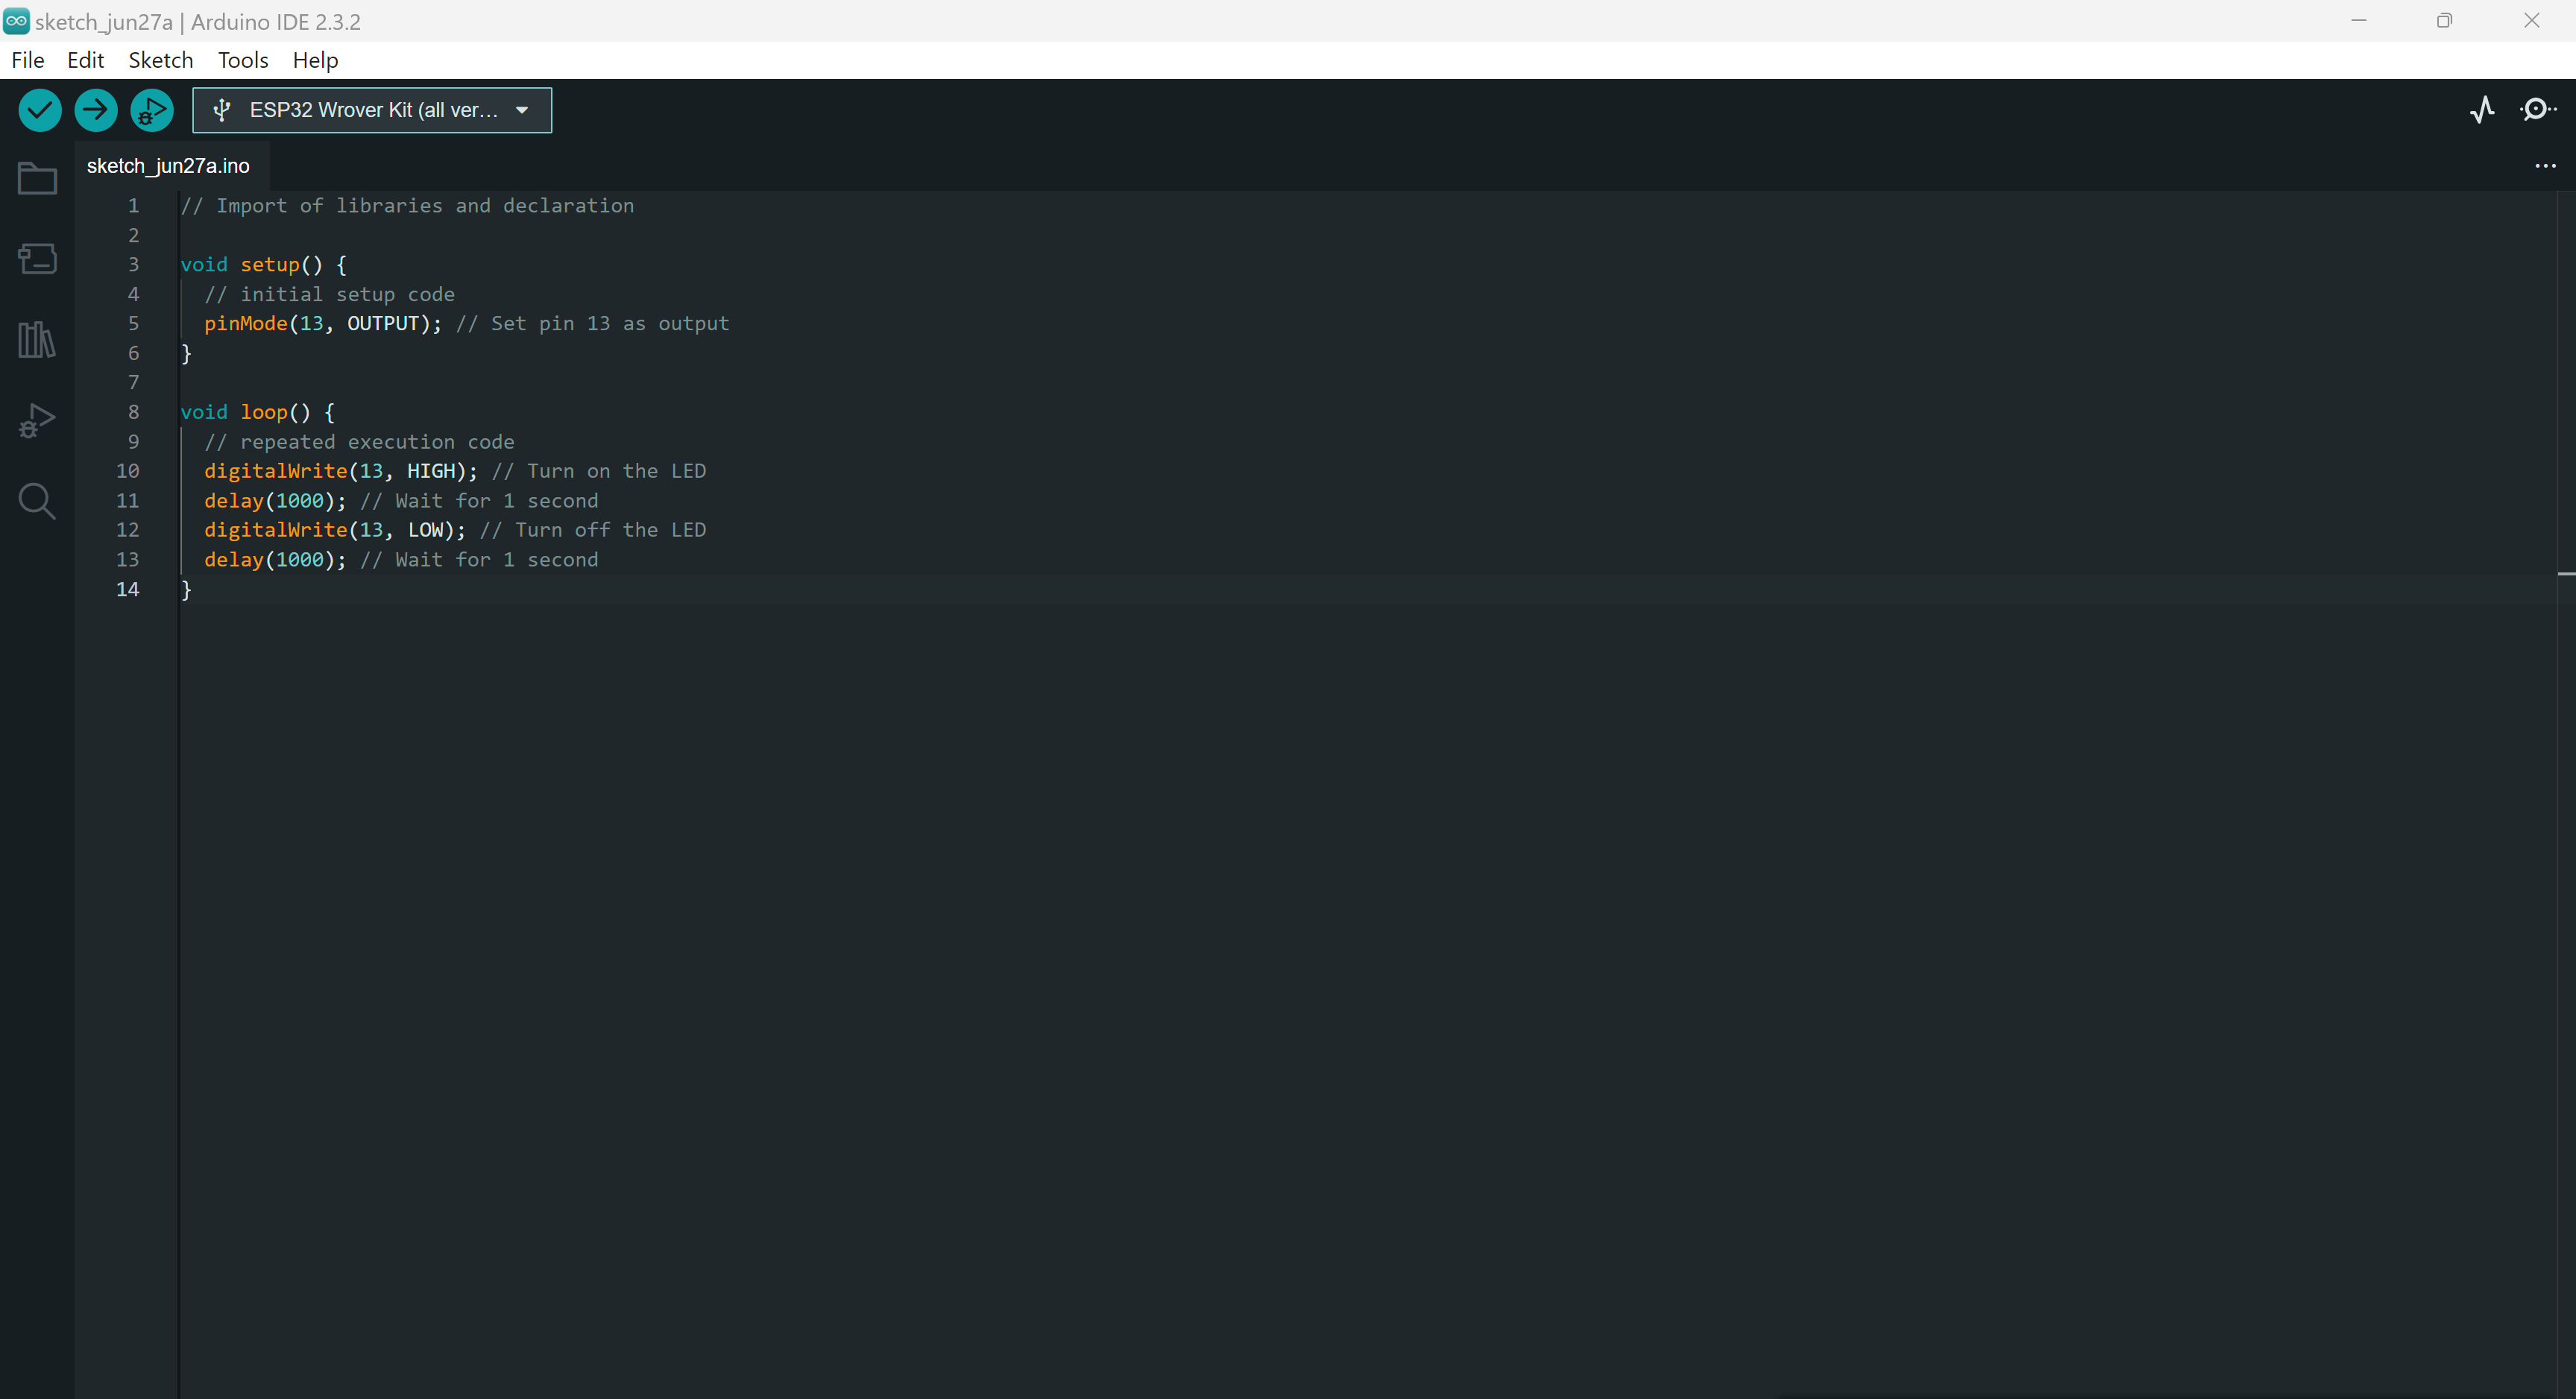
\includegraphics[width=\textwidth]{fig/fig19.png}
	\caption{C++ Syntax}
	\label{fig:19}
\end{figure}


\section{C++ Output}
\textbf{Teori:} Output i Arduino opnås ved at bruge \texttt{Serial.print()} og \texttt{Serial.println()} til at sende data til serial monitoren. Serial kommunikation er en vigtig funktion, som gør det muligt at kommunikere mellem Arduino og en computer. Dette er især nyttigt til debugging og overvågning af sensorværdier.
\newline\newline
\noindent\textbf{Serial Monitor:} Serial Monitor er et værktøj i Arduino IDE (Integrated Development Environment), der giver brugeren mulighed for at interagere med Arduino-boardet via seriel kommunikation. Når en Arduino er tilsluttet en computer via USB-kabel, kan den sende og modtage data til og fra computeren. Serial Monitor viser disse data i et tekstvindue og giver brugeren mulighed for at sende tekstdata til Arduinoen.
\newline\newline
\noindent Serial Monitor bruges ofte til følgende formål:
\begin{itemize}
	\item \textbf{Debugging:} Ved at bruge \texttt{Serial.print()} og \texttt{Serial.println()} kan programmører indsætte debugging-meddelelser i deres kode for at overvåge, hvad der sker i programmet. Dette gør det lettere at identificere og rette fejl.
	
	\item \textbf{Overvågning af sensorværdier:} Arduino kan læse data fra forskellige sensorer (f.eks. temperatur, lys, fugtighed) og sende disse data til Serial Monitor for at give en realtidsvisning af sensorens output.
	
	\item \textbf{Brugerinput:} Brugere kan sende kommandoer eller data fra Serial Monitor til Arduino. Dette er nyttigt til at ændre parametre i programmet uden at skulle uploade ny kode til Arduinoen.
	
	\item \textbf{Kommunikation:} Serial Monitor kan bruges til at kommunikere med andre serielle enheder, som er tilsluttet Arduinoen, såsom GPS-moduler, GSM-moduler, og andre mikrocontrollere.
\end{itemize}
\noindent\textbf{Eksempel: Output til Seriel Monitor}
\begin{lstlisting}[language=C++]
	void setup() {
		Serial.begin(9600); // Initialize serial communication at 9600 baud
	}
	
	void loop() {
		Serial.println("Hello, Arduino!");
		delay(1000); // wait for a second
	}
\end{lstlisting}
\clearpage
\begin{figure}[h!]
	\centering
	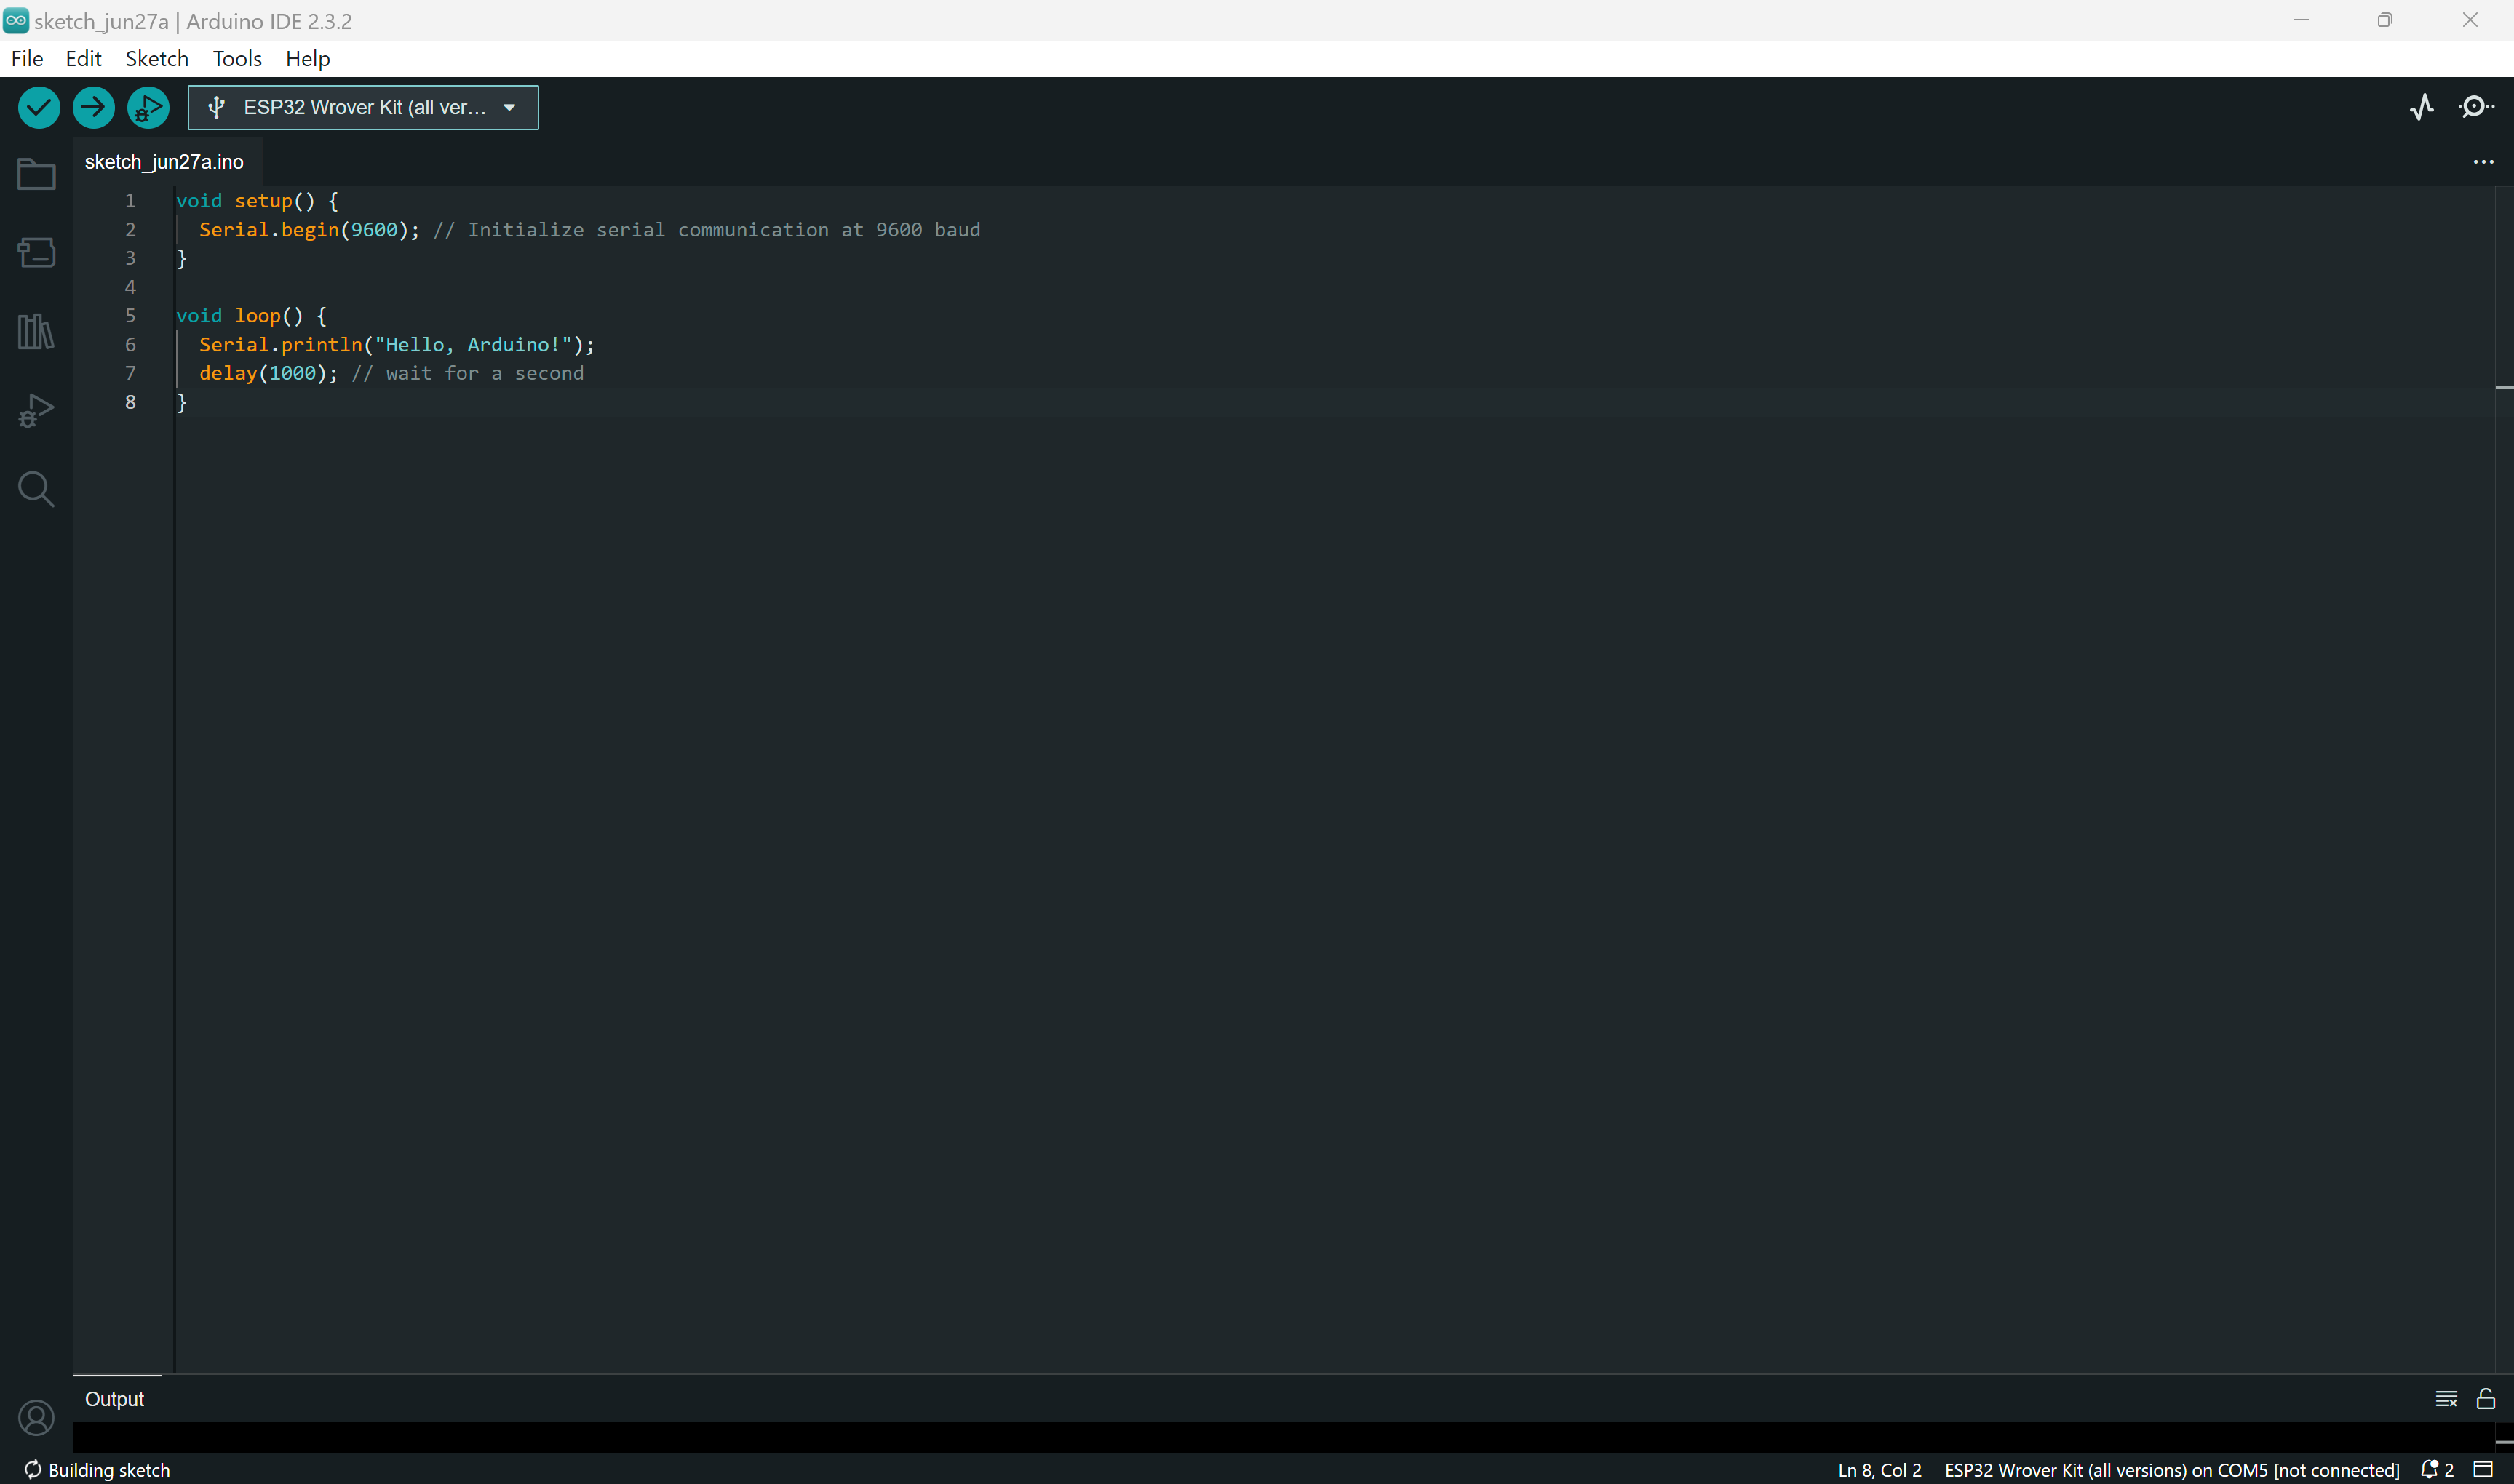
\includegraphics[width=\textwidth]{fig/fig1.png}
	\caption{C++ Output}
	\label{fig:1}
\end{figure}

\noindent\textbf{Eksempel: Seriel Monitor for debugging}
\begin{lstlisting}[language=C++]
	void setup() {
		Serial.begin(9600); // Initialize serial communication at 9600 baud
	}
	
	void loop() {
		int sensorValue = analogRead(A0);
		Serial.print("Sensor Value: ");
		Serial.println(sensorValue);
	}
\end{lstlisting}
\clearpage
\begin{figure}[h!]
	\centering
	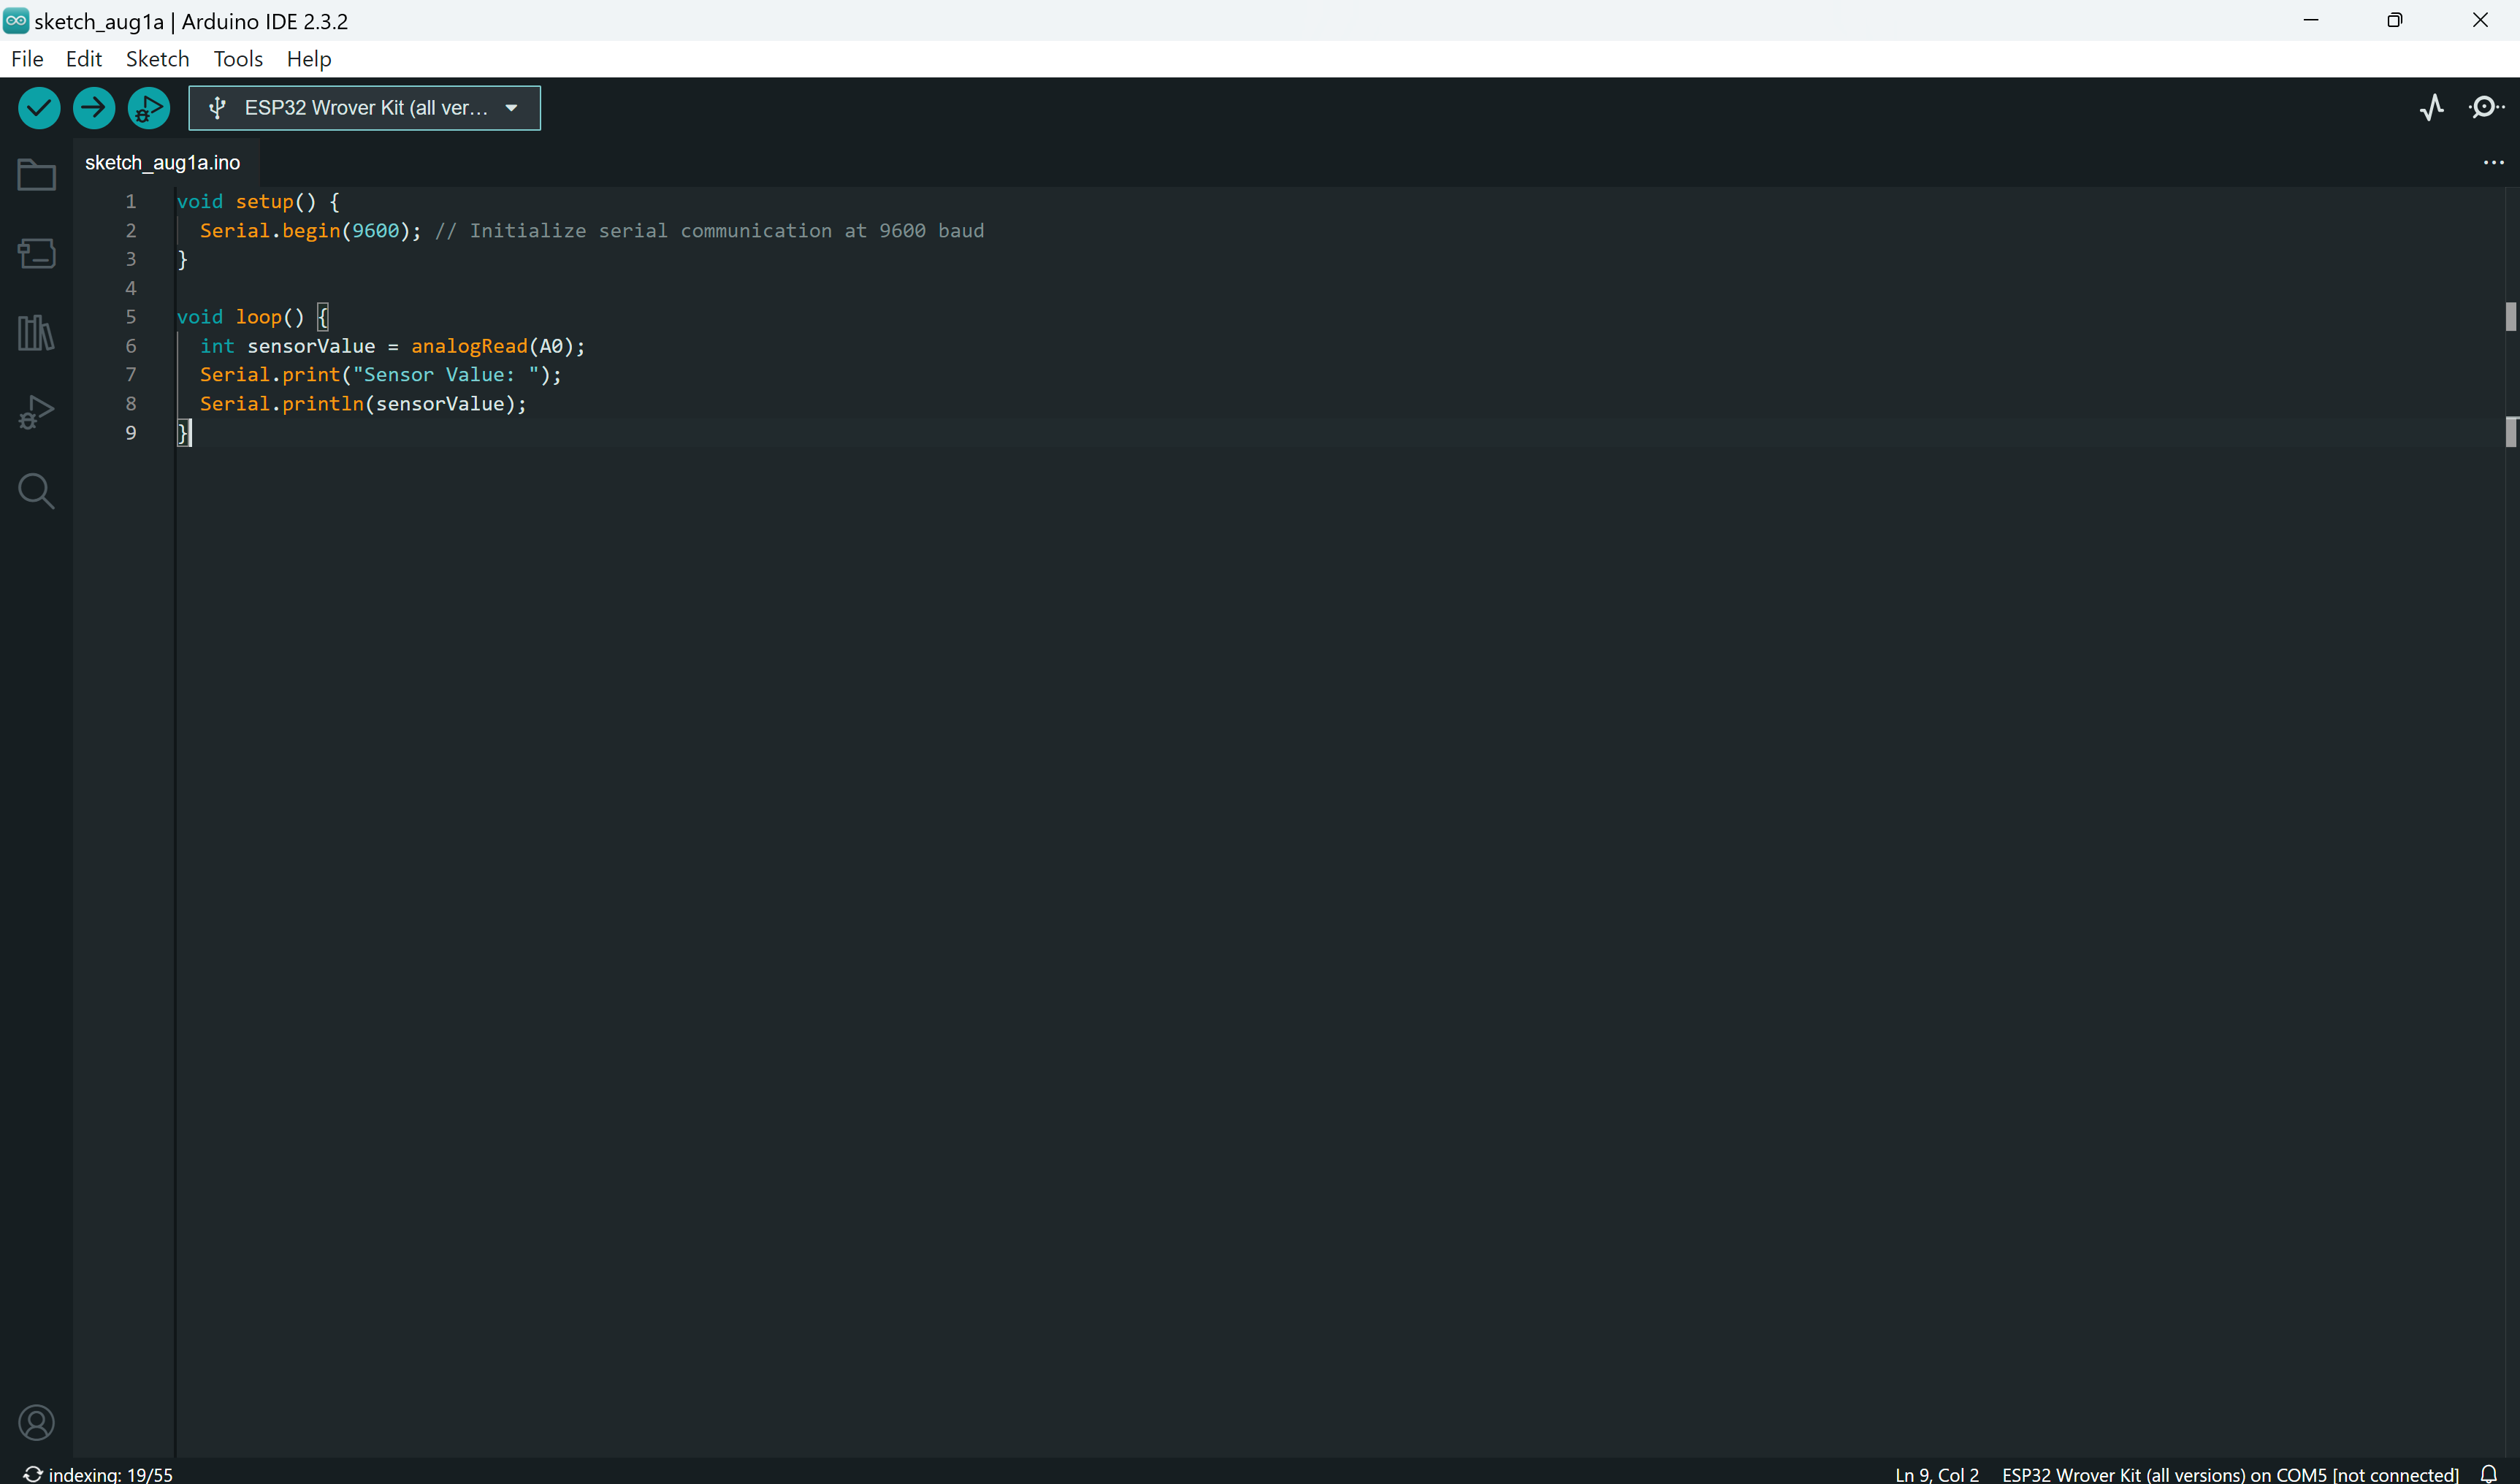
\includegraphics[width=\textwidth]{fig/fig21.png}
	\caption{C++ Output}
	\label{fig:21}
\end{figure}

\section{C++ Comments}
\textbf{Teori:} Kommentarer bruges til at dokumentere koden og forklare, hvad de forskellige dele af programmet gør. De ignoreres af compileren og gør det lettere for andre (og dig selv) at forstå koden senere.
\begin{itemize}
	\item Hvis \texttt{//} bruges, så laves en kommentar for en enkelt linje.
	\item Hvis \texttt{/* */} bruges, vil alt imellem \texttt{/*} og \texttt{*/} blive betragtet som en kommentar.
\end{itemize}
Udover at blive brugt til at lave kommentarer, kan de også bruges til at debugge koden ved midlertidigt at deaktivere visse dele af programmet.
\clearpage
\noindent\textbf{Eksempel:}
\begin{lstlisting}[language=C++]
	// This is a single line comment
	/*
	This is a block comment
	that spans multiple lines
	*/
	void setup() {
		// Initialize pin 13 as an output
		pinMode(13, OUTPUT);
	}
\end{lstlisting}
\begin{figure}[h!]
	\centering
	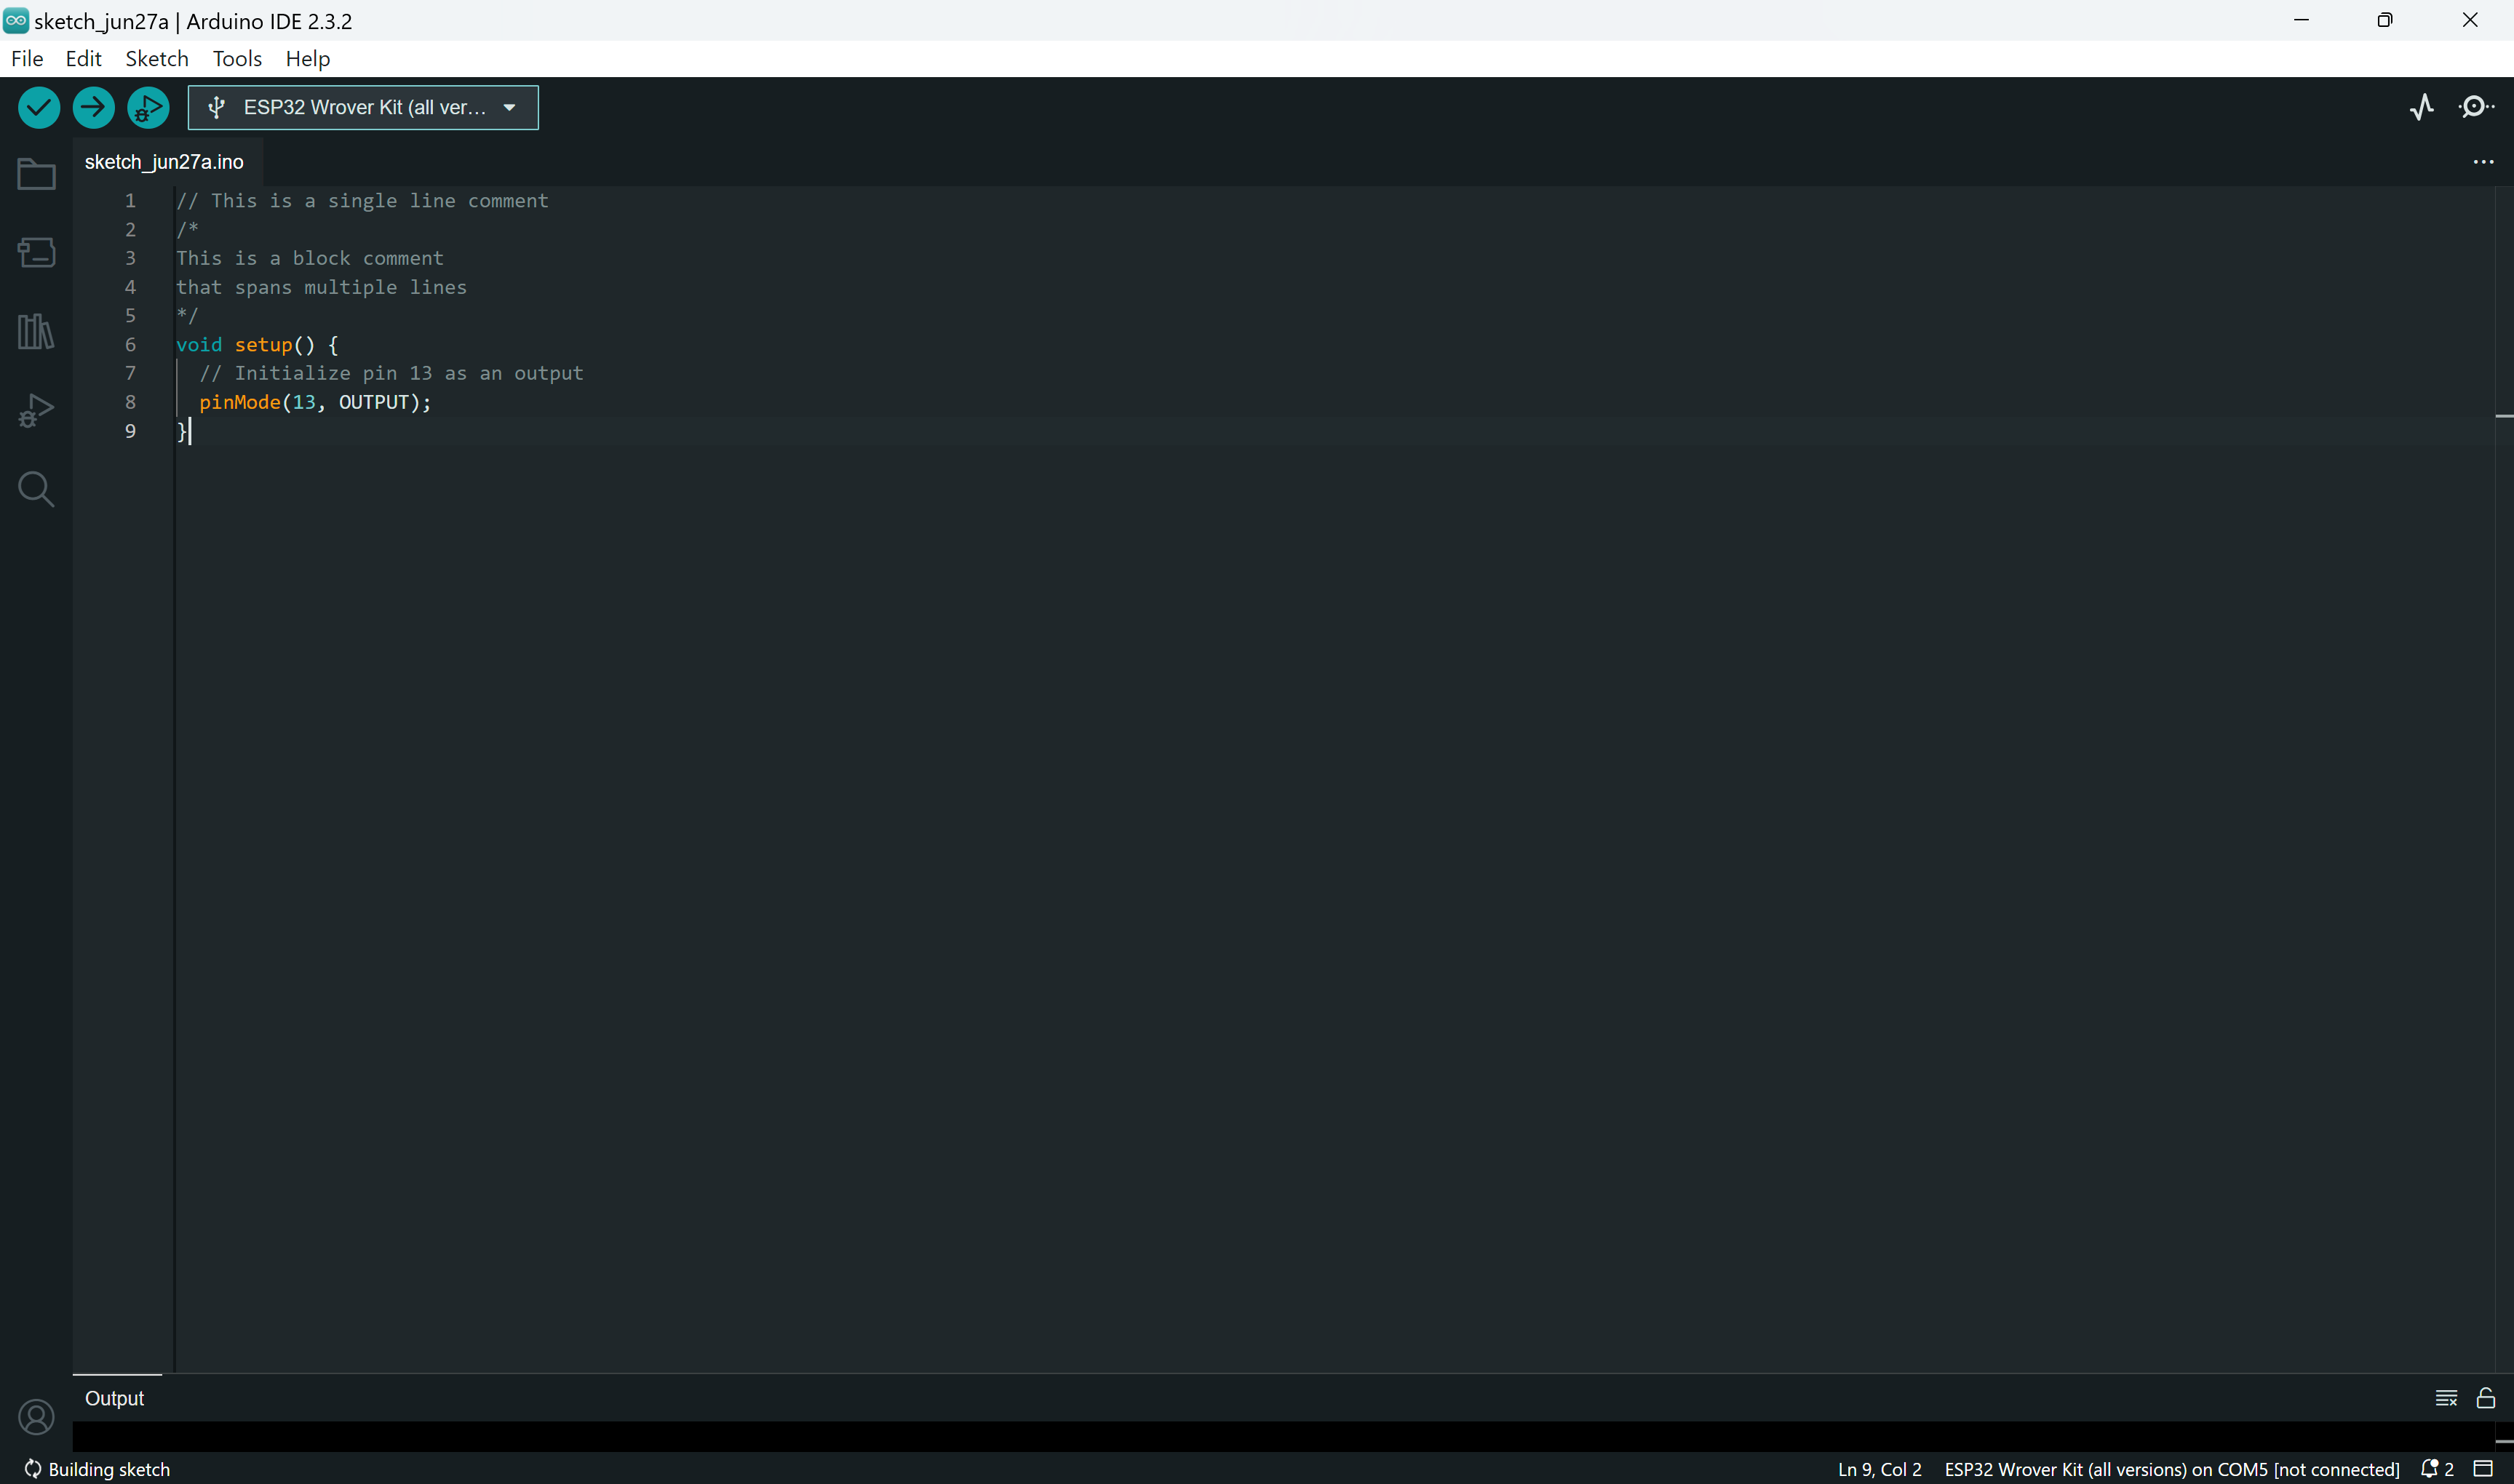
\includegraphics[width=\textwidth]{fig/fig2.png}
	\caption{C++ Comments}
	\label{fig:2}
\end{figure}

\section{C++ Variables}
\textbf{Teori:} Variabler bruges til at gemme data, der kan ændres under programmets kørsel. Variabler skal deklareres med en datatype før brug. Typiske datatyper inkluderer \texttt{int}, \texttt{float}, \texttt{char}, og \texttt{bool}.
\clearpage
\noindent\textbf{Eksempel:}
\begin{lstlisting}[language=C++]
	int ledPin = 13; // declare an integer variable
	
	void setup() {
		pinMode(ledPin, OUTPUT); // use the variable
	}
	
	void loop() {
		digitalWrite(ledPin, HIGH); // turn the LED on
		delay(1000);
		digitalWrite(ledPin, LOW); // turn the LED off
		delay(1000);
	}
\end{lstlisting}
\begin{figure}[h!]
	\centering
	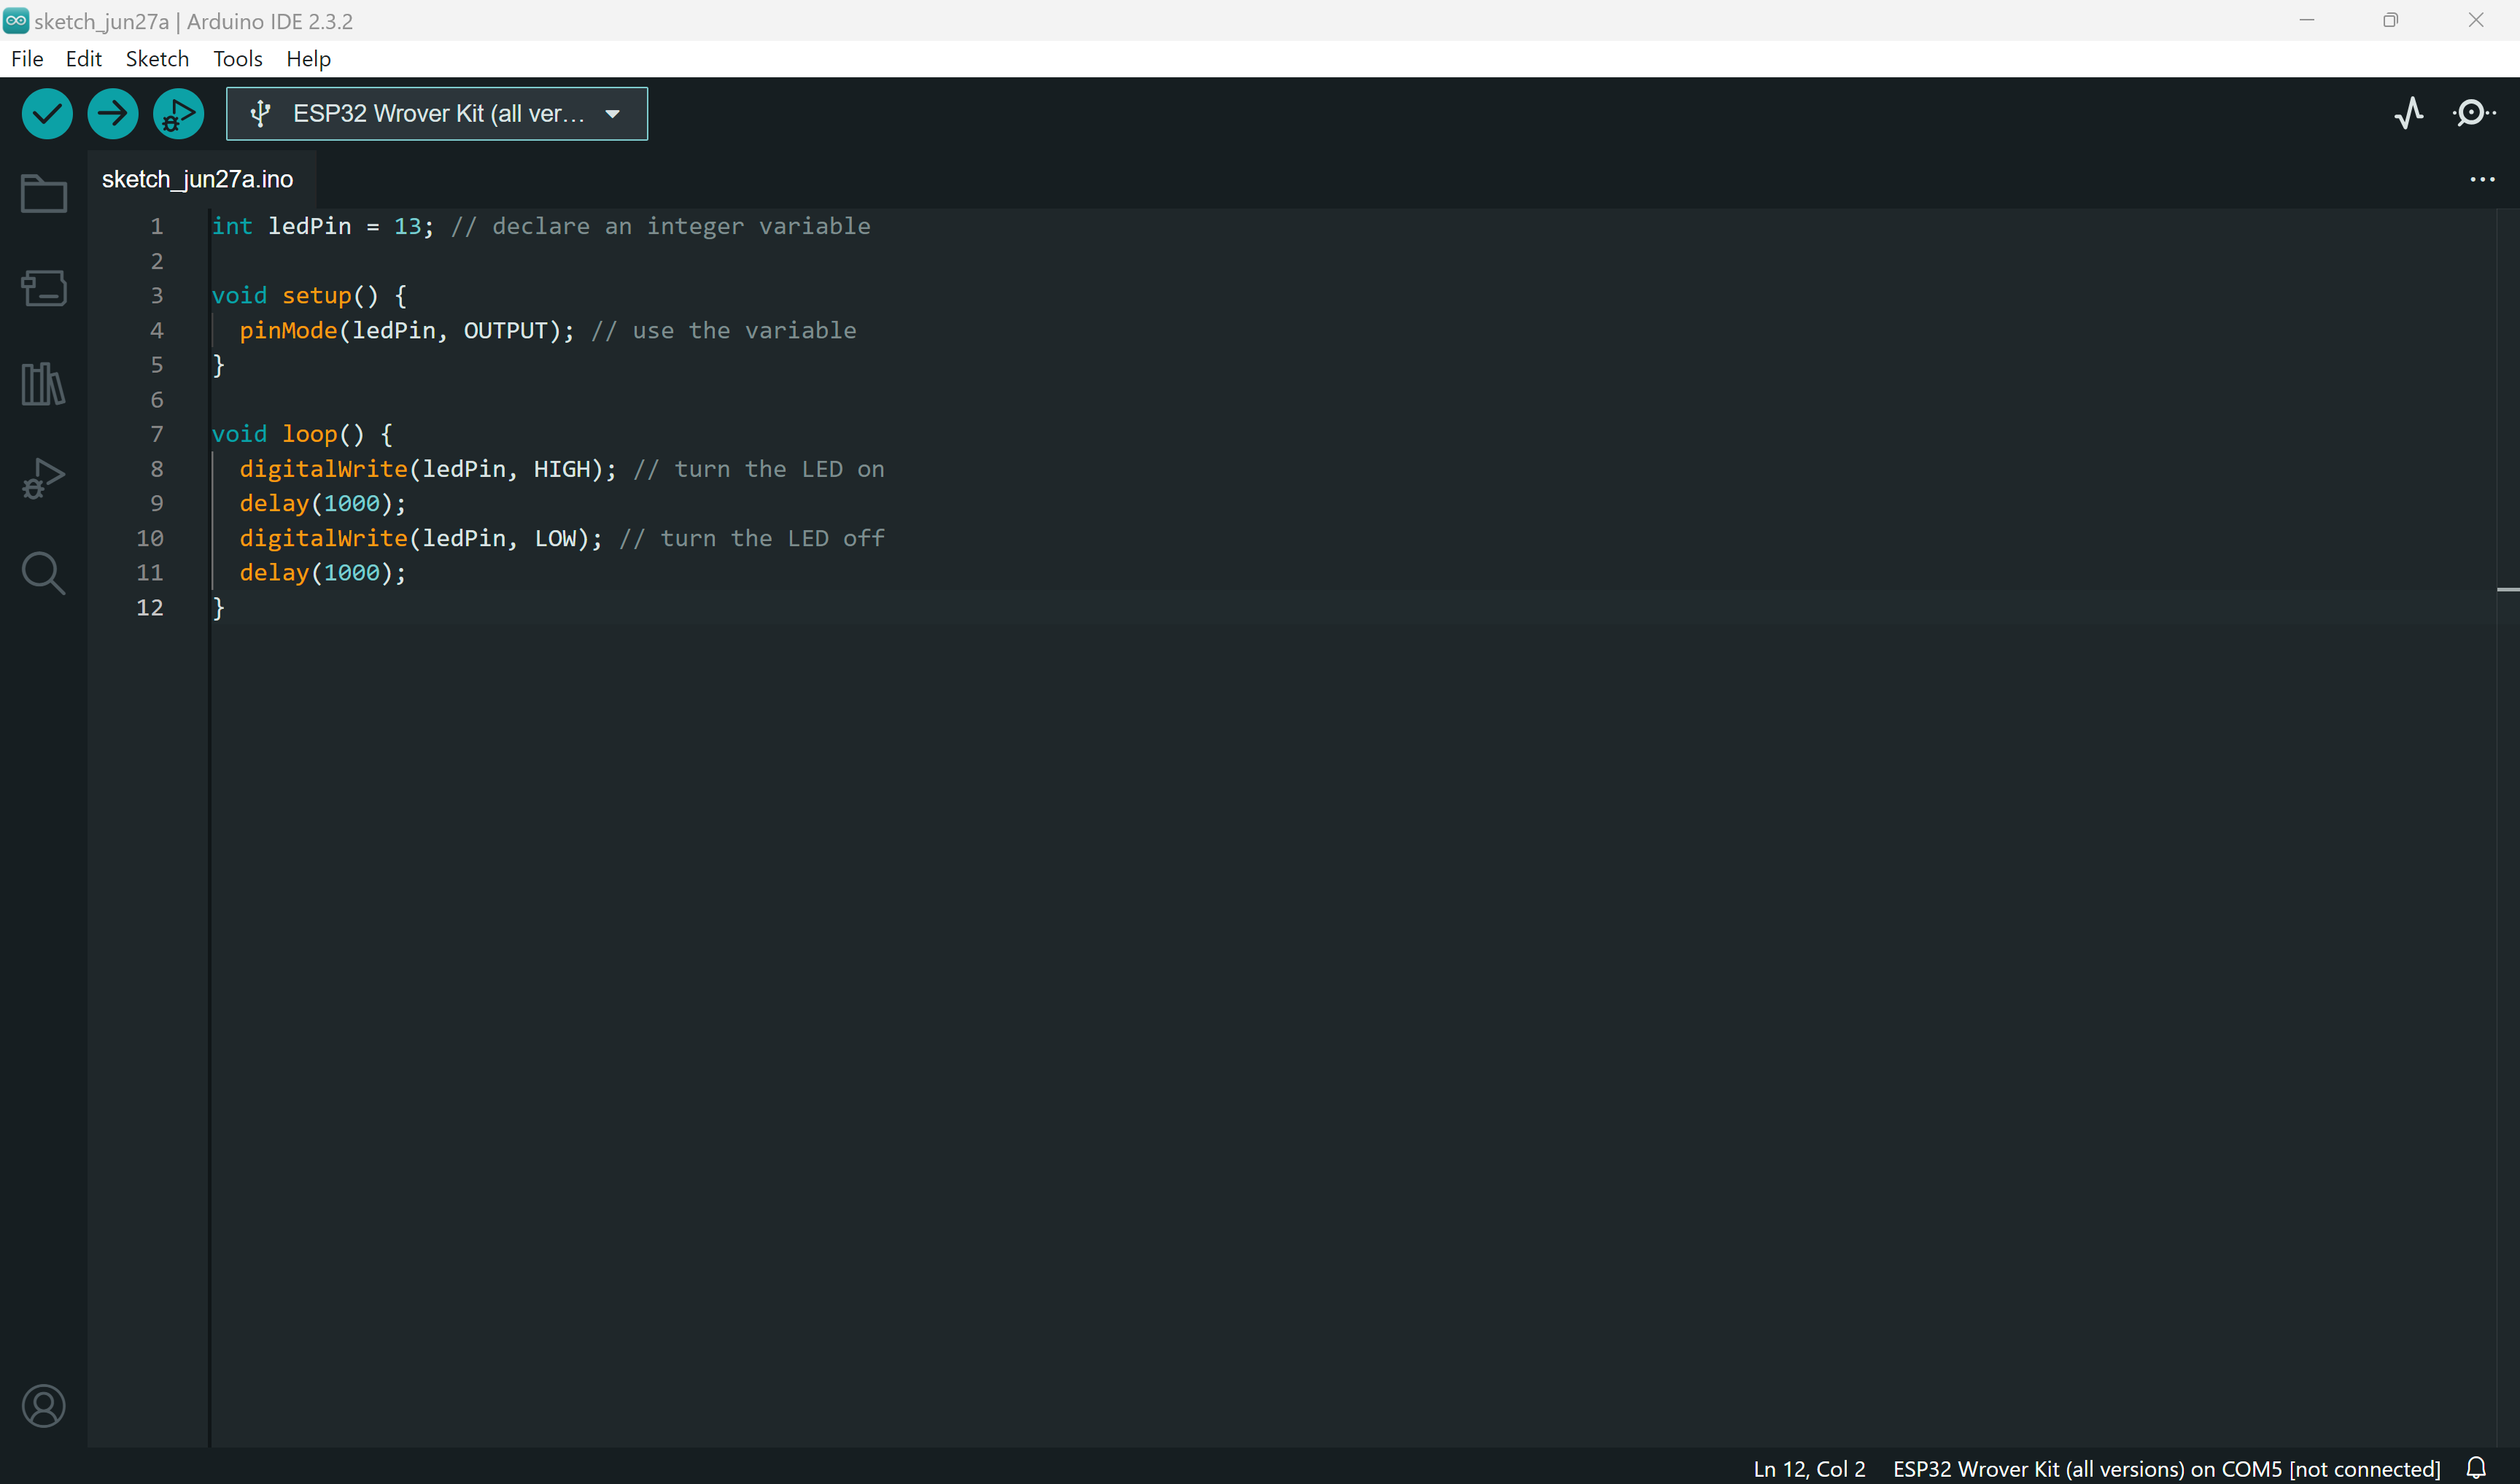
\includegraphics[width=\textwidth]{fig/fig3.png}
	\caption{C++ Variables}
	\label{fig:3}
\end{figure}

\noindent\textbf{Navnekonventioner for Variabler}
Når man skriver kode, er det vigtigt at følge nogle navnekonventioner for variabler for at gøre koden læsbar og nemmere at vedligeholde. Her er nogle almindelige navnekonventioner:
\begin{itemize}
	\item \textbf{camelCase}: Begynder med et lille bogstav, og hvert efterfølgende ord starter med et stort bogstav. Eksempel: \texttt{sensorValue}, \texttt{scaledValue}.
	\item \textbf{PascalCase}: Hvert ord starter med et stort bogstav. \\Eksempel: \texttt{SensorValue}, 
	\texttt{ScaledValue}.
	\item \textbf{snake\_case}: Alle bogstaver er små, og ord adskilles med underscores. Eksempel: 
	\texttt{sensor\_value}, \texttt{scaled\_value}.
	\item \textbf{kebab-case}: Alle bogstaver er små, og ord adskilles med bindestreger (bruges sjældent i programmeringssprog som C++). \\Eksempel:
	\texttt{sensor-value}, \texttt{scaled-value}.
\end{itemize}

\section{C++ User Input}
\textbf{Teori:} Brugerinput modtages via sensorer eller knapper og behandles med \texttt{analogRead()} og \texttt{digitalRead()} funktioner. Disse funktioner gør det muligt for Arduino at interagere med omgivelserne. \texttt{analogRead(pin)} læser en værdi mellem 0 og 1023 fra en analog pin, mens \texttt{digitalRead(pin)} læser enten HIGH eller LOW fra en digital pin.
\newline\newline
\noindent\textbf{Eksempel:}
\begin{lstlisting}[language=C++]
	int sensorPin = A0; // select the input pin for the sensor
	int sensorValue = 0; // variable to store the value coming from the sensor
	
	void setup() {
		Serial.begin(9600); // initialize serial communication
	}
	
	void loop() {
		sensorValue = analogRead(sensorPin); // read the value from the sensor
		Serial.println(sensorValue); // print the value to the serial monitor
		delay(1000); // wait for a second
	}
\end{lstlisting}
\clearpage
\begin{figure}[t!]
	\centering
	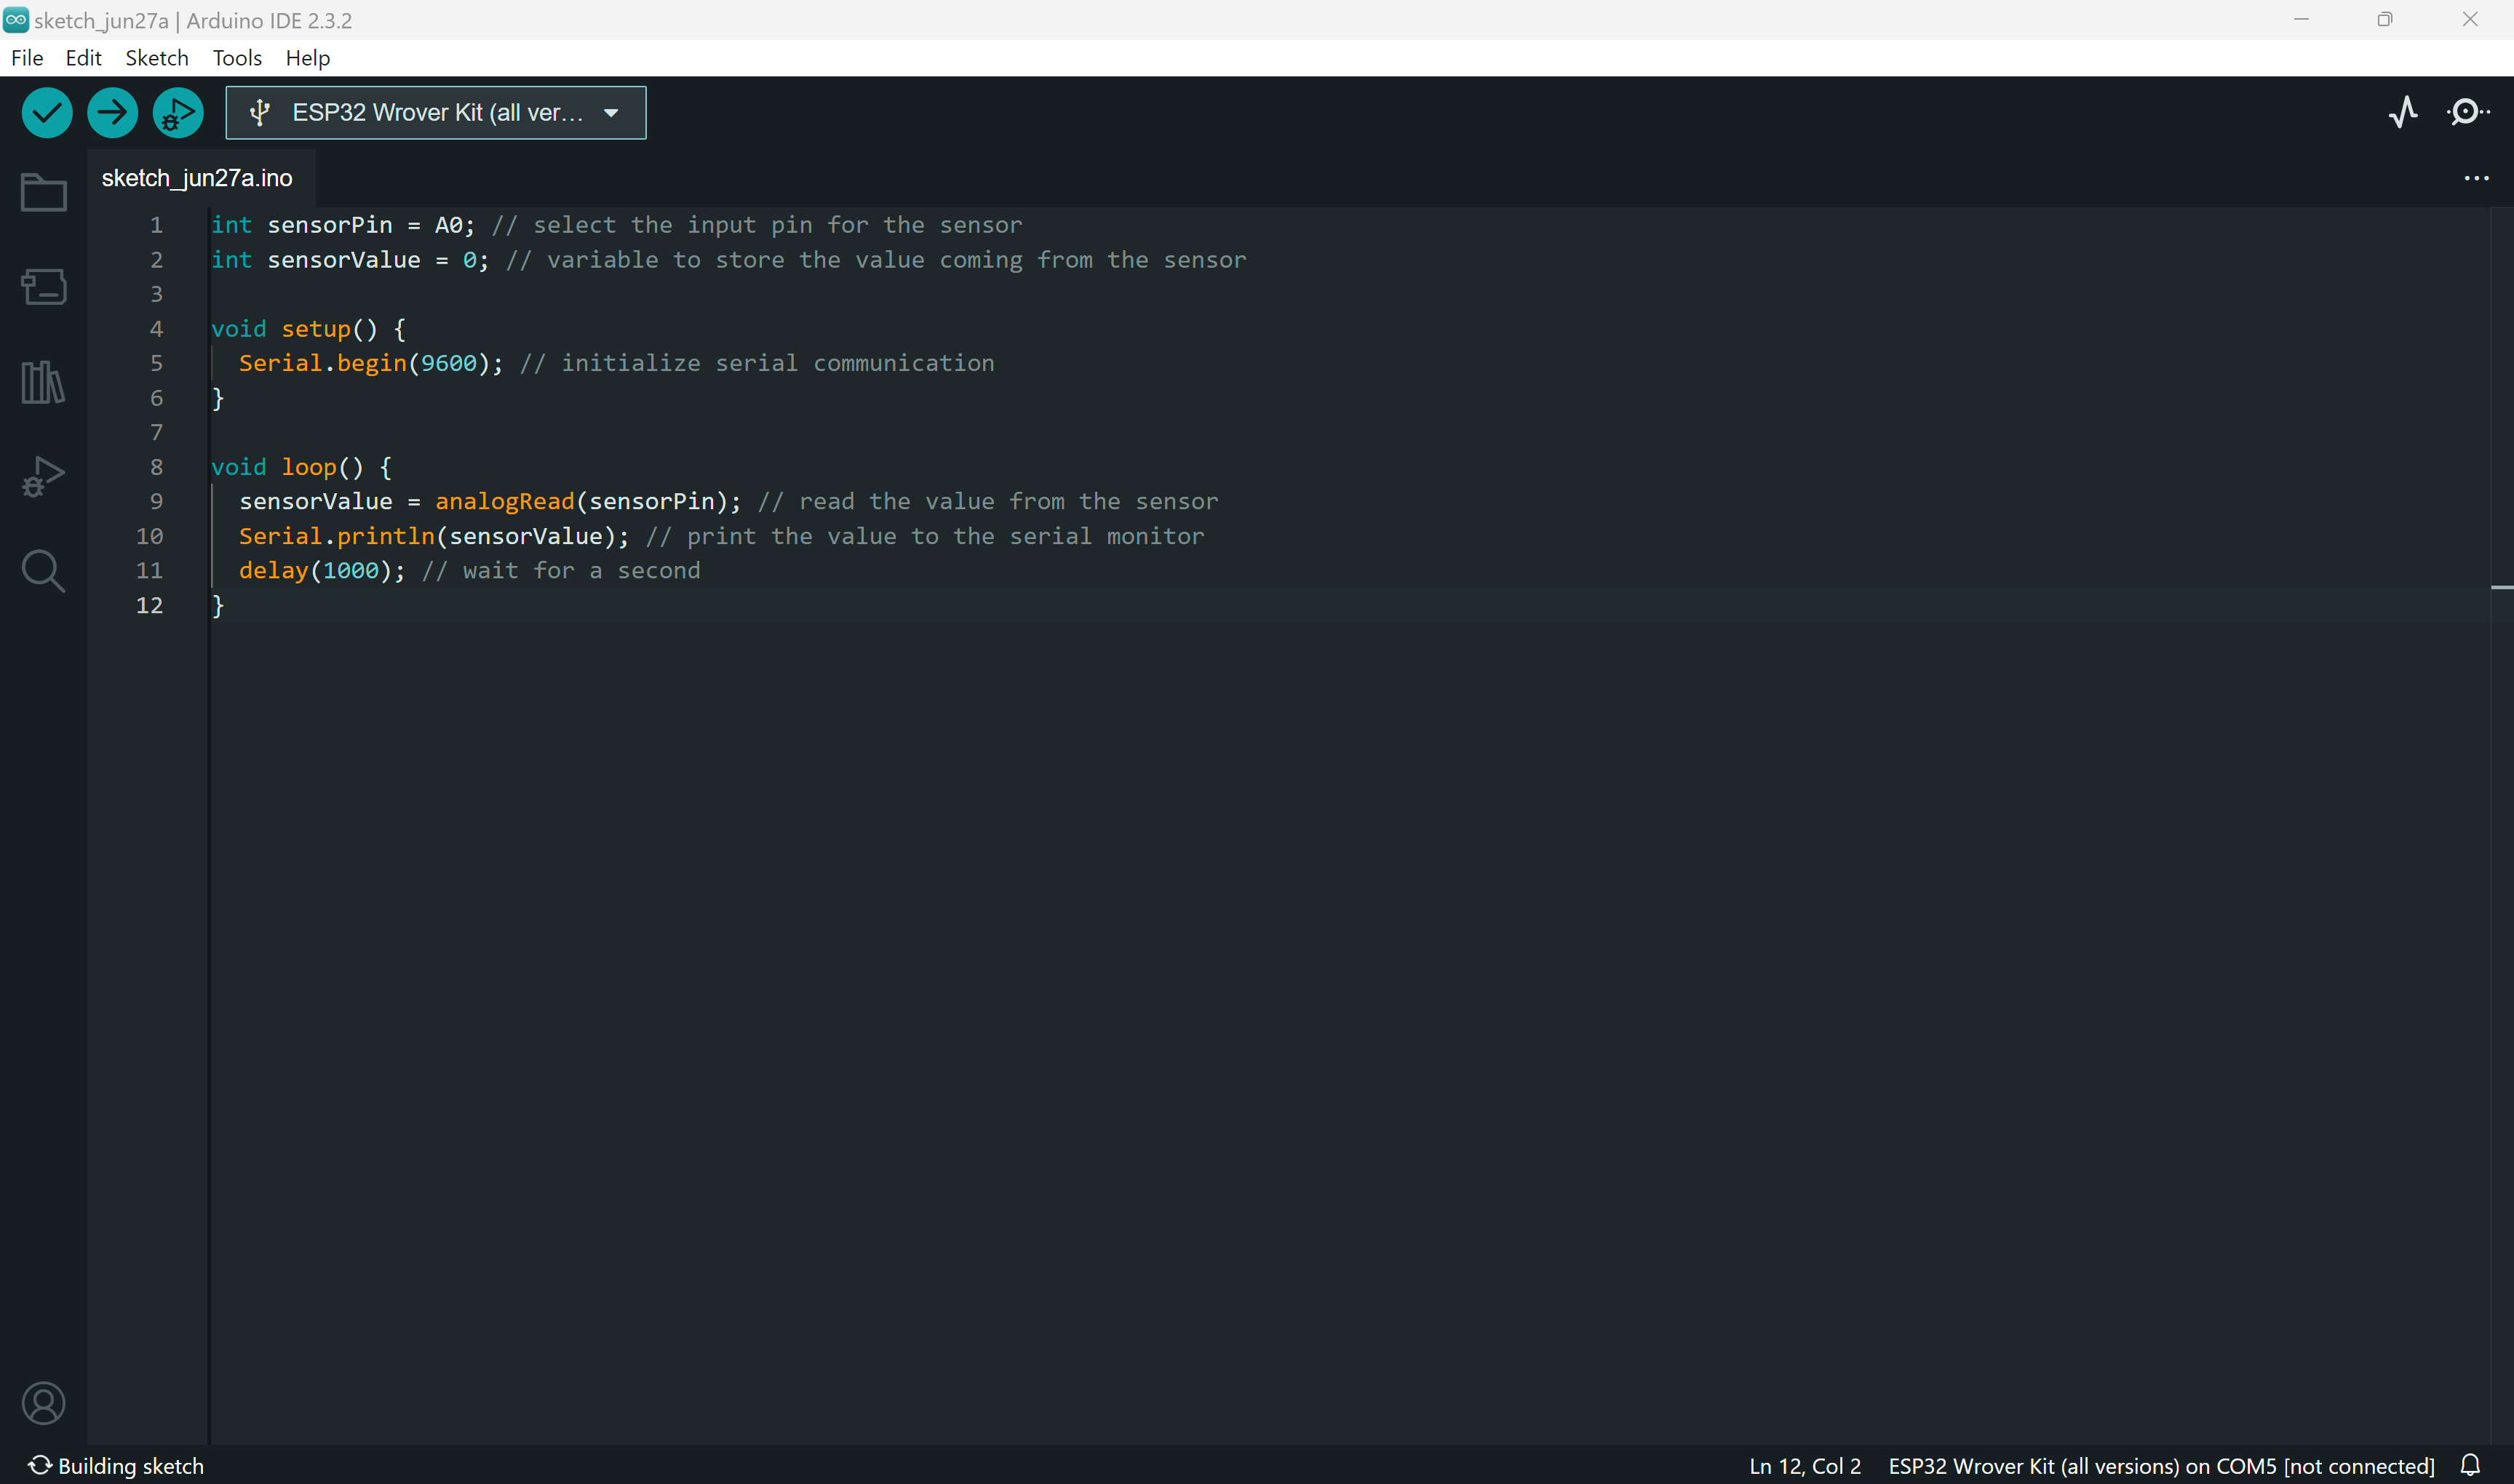
\includegraphics[width=\textwidth]{fig/fig4.png}
	\caption{C++ User Input}
	\label{fig:4}
\end{figure}
\section{C++ Data Types}
\textbf{Teori:} Data typer i C++ definerer den type data en variabel kan holde. Almindelige datatyper inkluderer \texttt{int} (heltal), \texttt{float} (flydende punkt tal), \texttt{char} (karakter), og \texttt{bool} (boolean, sand/falsk). Valg af korrekt datatype er vigtig for at optimere hukommelsesbrug og præcision.Variabler kan initialiseres ved deklaration eller senere i programmet. Liste over de mest gængse datatyper:
\begin{table}[h!]
	\centering
	\tiny
	\begin{tabular}{|l|l|l|l|l|l|}
		\hline
		\texttt{char}&1 byte& -128 til 127&\texttt{int}&4 bytes&-32,768 til 32,767\\\hline
		\texttt{float}&4 bytes&3.40E-38 til 3.40E+38&\texttt{double}&8 bytes&3.402E-38 to 3.402E+38\\\hline
		\texttt{boolean}& 1 byte& 0 til 1& word &4 bytes& 0 til 65,535\\\hline
	\end{tabular}
\end{table}
\clearpage
\noindent\textbf{Eksempel:}
\begin{lstlisting}[language=C++]
	int ledPin = 13;
	float voltage = 5.0;
	char myChar = 'A';
	bool isOn = true;
	
	void setup() {
		Serial.begin(9600);
		Serial.println(voltage);
	}
	
	void loop() {
		if (isOn) {
			digitalWrite(ledPin, HIGH);
		} else {
			digitalWrite(ledPin, LOW);
		}
		delay(1000);
	}
\end{lstlisting}

\begin{figure}[!h]
	\centering
	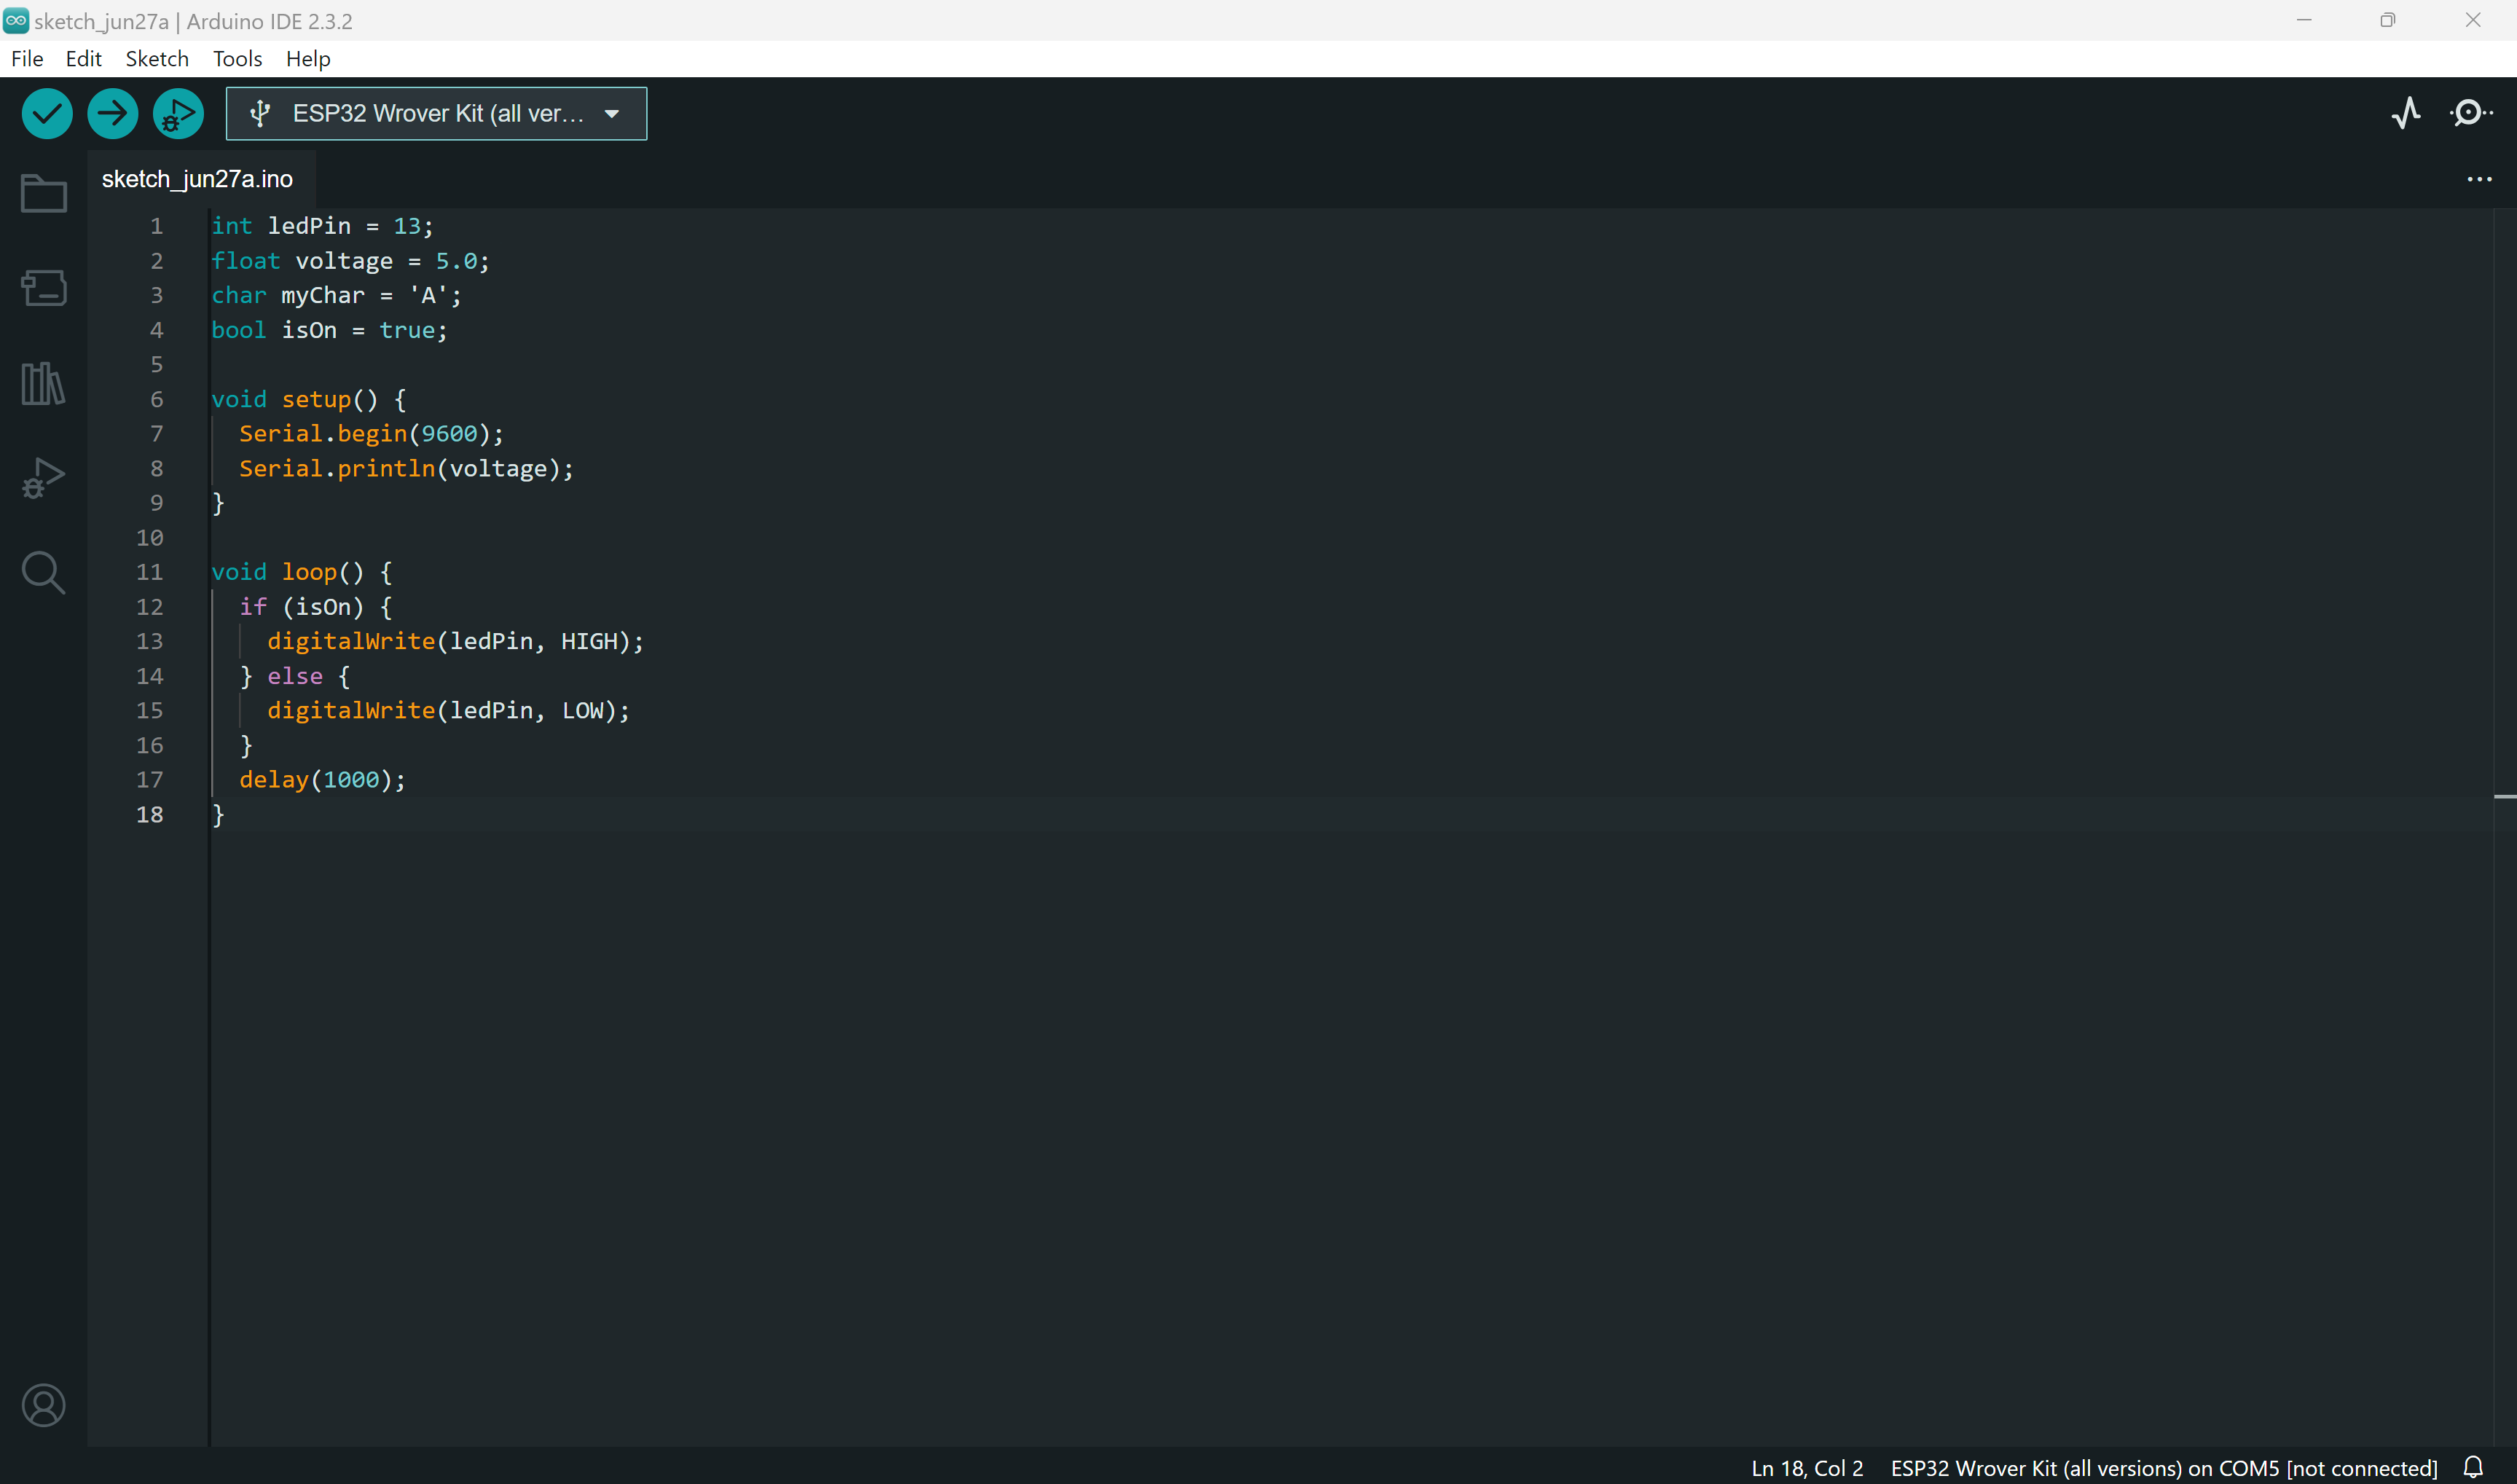
\includegraphics[width=\textwidth]{fig/fig5.png}
	\caption{C++ Data Types}
	\label{fig:5}
\end{figure}

\section{C++ Operators}
\textbf{Teori:} Operatorer bruges til at udføre operationer på variabler og værdier. Aritmetiske operatorer (\texttt{+}, \texttt{-}, \texttt{*}, \texttt{/}) bruges til matematiske operationer. Logiske operatorer (\texttt{\&\&}, \texttt{||}, \texttt{!}) bruges til at kombinere eller negere betingelser. Tildelingsoperatoren (\texttt{=}) bruges til at tildele værdier til variabler.
\newline\newline
\noindent\textbf{Eksempel:}
\begin{lstlisting}[language=C++]
	int a = 5;
	int b = 10;
	int sum = a + b;
	bool result = (a < b) && (b > 0);
	
	void setup() {
		Serial.begin(9600);
		Serial.println(sum);
		Serial.println(result);
	}
	
	void loop() {
		// empty loop
	}
\end{lstlisting}
\begin{figure}[h!]
	\centering
	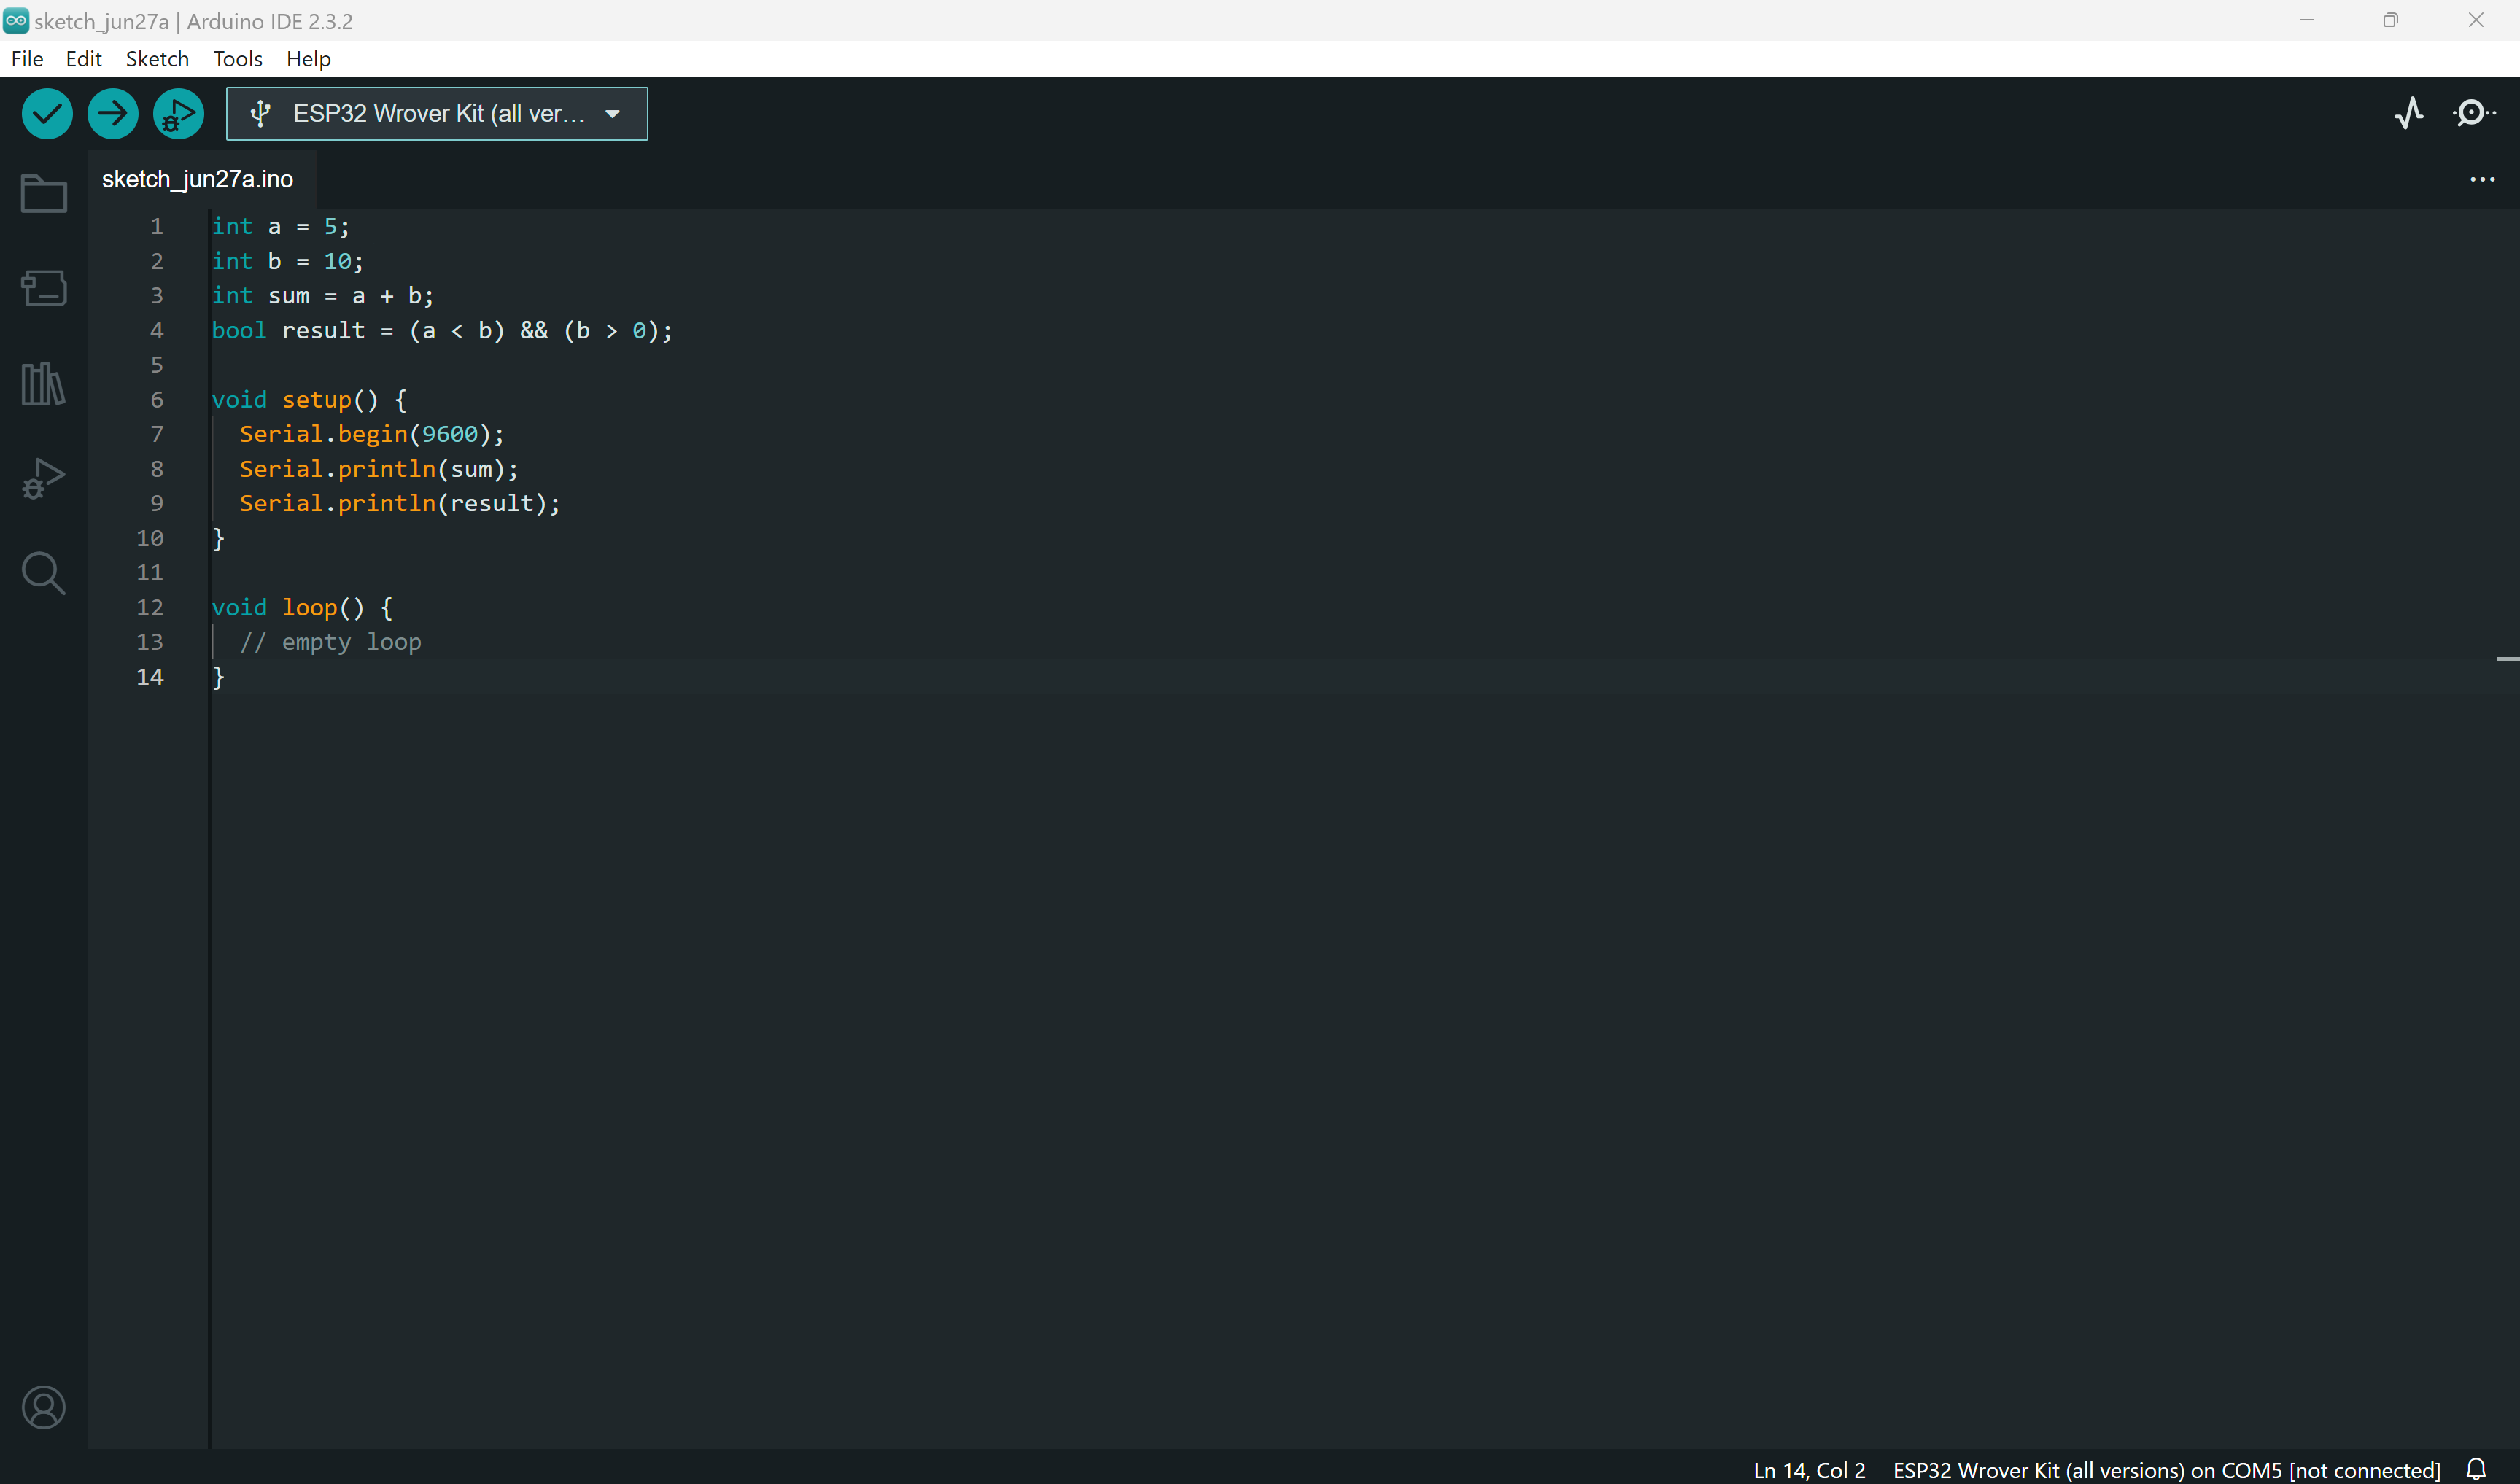
\includegraphics[width=\textwidth]{fig/fig6.png}
	\caption{C++ Operators}
	\label{fig:6}
\end{figure}

\section{C++ Strings}
\textbf{Teori:} Strings i C++ bruges til at holde tekst. De kan håndteres ved hjælp af String klassen i Arduino. Strings kan konkateneres, sammenlignes, og manipuleres på forskellige måder. Stringmanipulation er nyttig til at formatere og vise tekstbaseret data.
\newline\newline
\noindent\textbf{Eksempel:}
\begin{lstlisting}[language=C++]
	String greeting = "Hello";
	String name = "Arduino";
	String message = greeting + ", " + name + "!";
	
	void setup() {
		Serial.begin(9600);
		Serial.println(message);
	}
	
	void loop() {
		// empty loop
	}
\end{lstlisting}
\begin{figure}[h!]
	\centering
	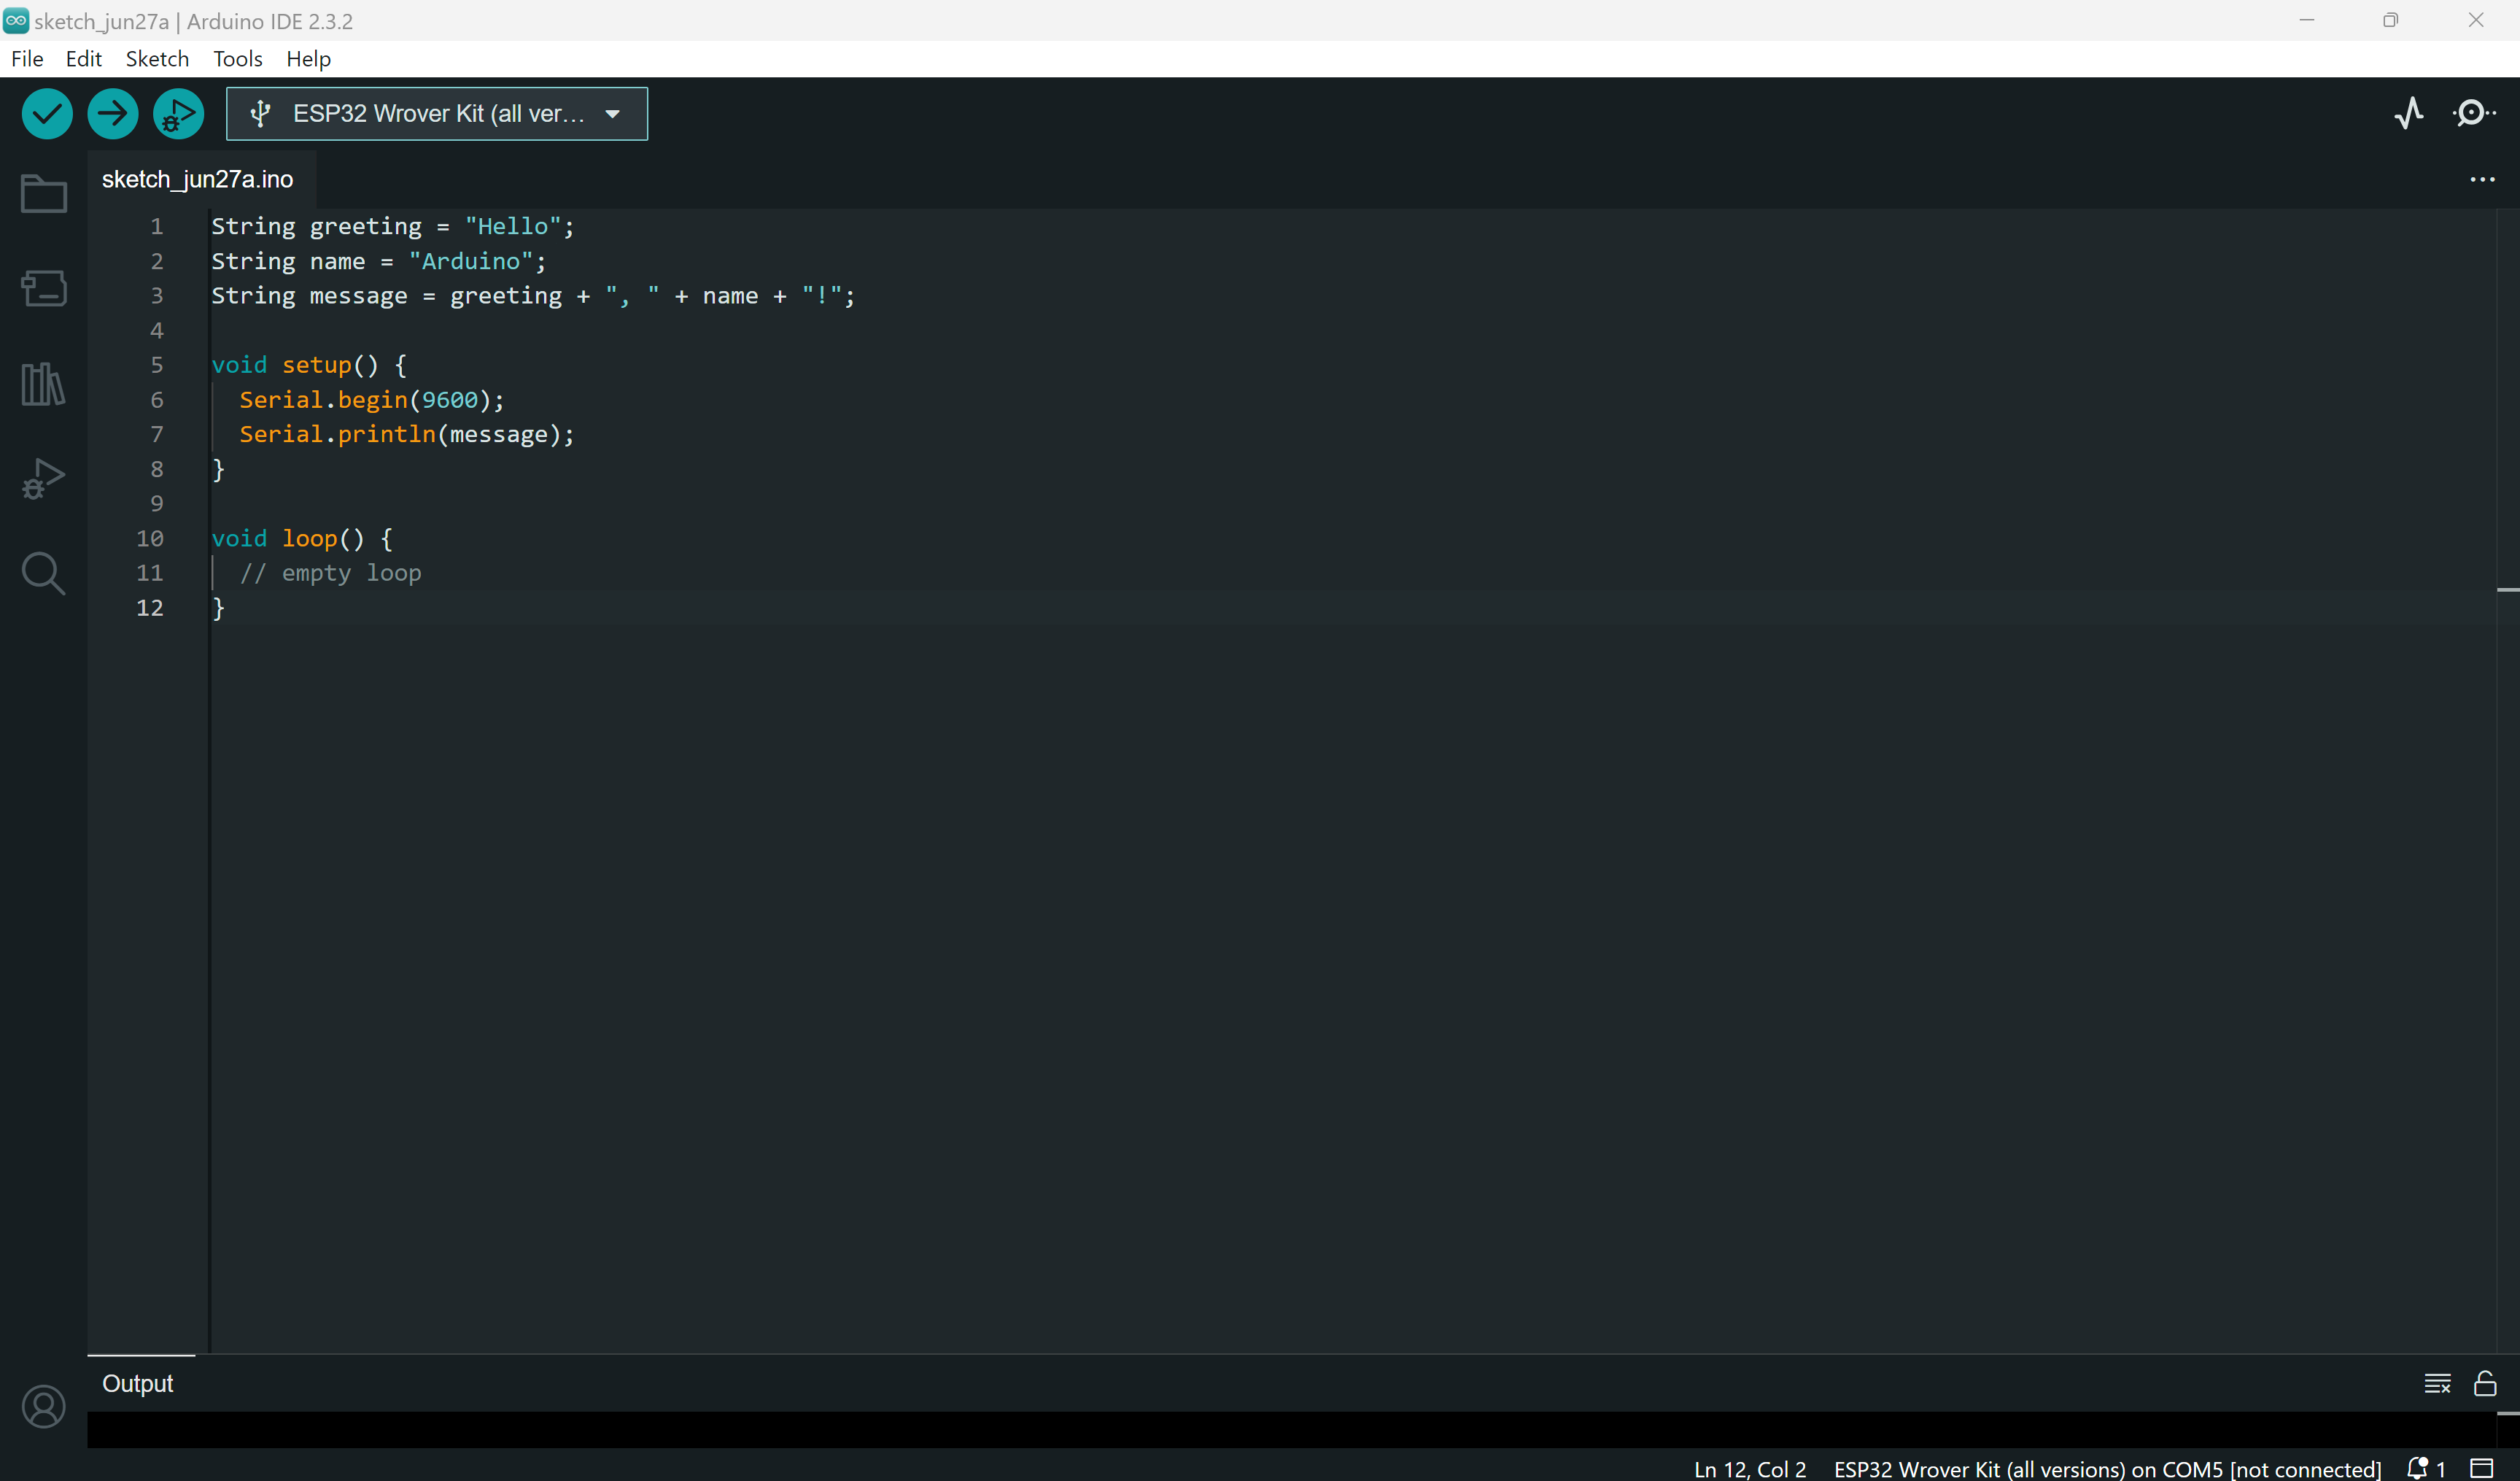
\includegraphics[width=\textwidth]{fig/fig7.png}
	\caption{C++ Strings}
	\label{fig:7}
\end{figure}

\section{C++ Conditions}
\textbf{Teori:} Betingede udsagn (if-else) bruges til at udføre forskellige handlinger baseret på forskellige betingelser. If-else strukturer tillader programmet at træffe beslutninger baseret på input eller tilstande. Komplekse beslutningstræer kan bygges ved at kombinere flere if-else udsagn. En anden betinget udsagn \texttt{case}.
\newline\newline
\noindent\textbf{Eksempel: \texttt{if}}
\begin{lstlisting}[language=C++]
	int sensorValue = 0;
	
	void setup() {
		Serial.begin(9600);
	}
	
	void loop() {
		sensorValue = analogRead(A0);
		if (sensorValue > 500) {
			Serial.println("High");
		} else {
			Serial.println("Low");
		}
		delay(1000);}
\end{lstlisting}
\begin{figure}[h!]
	\centering
	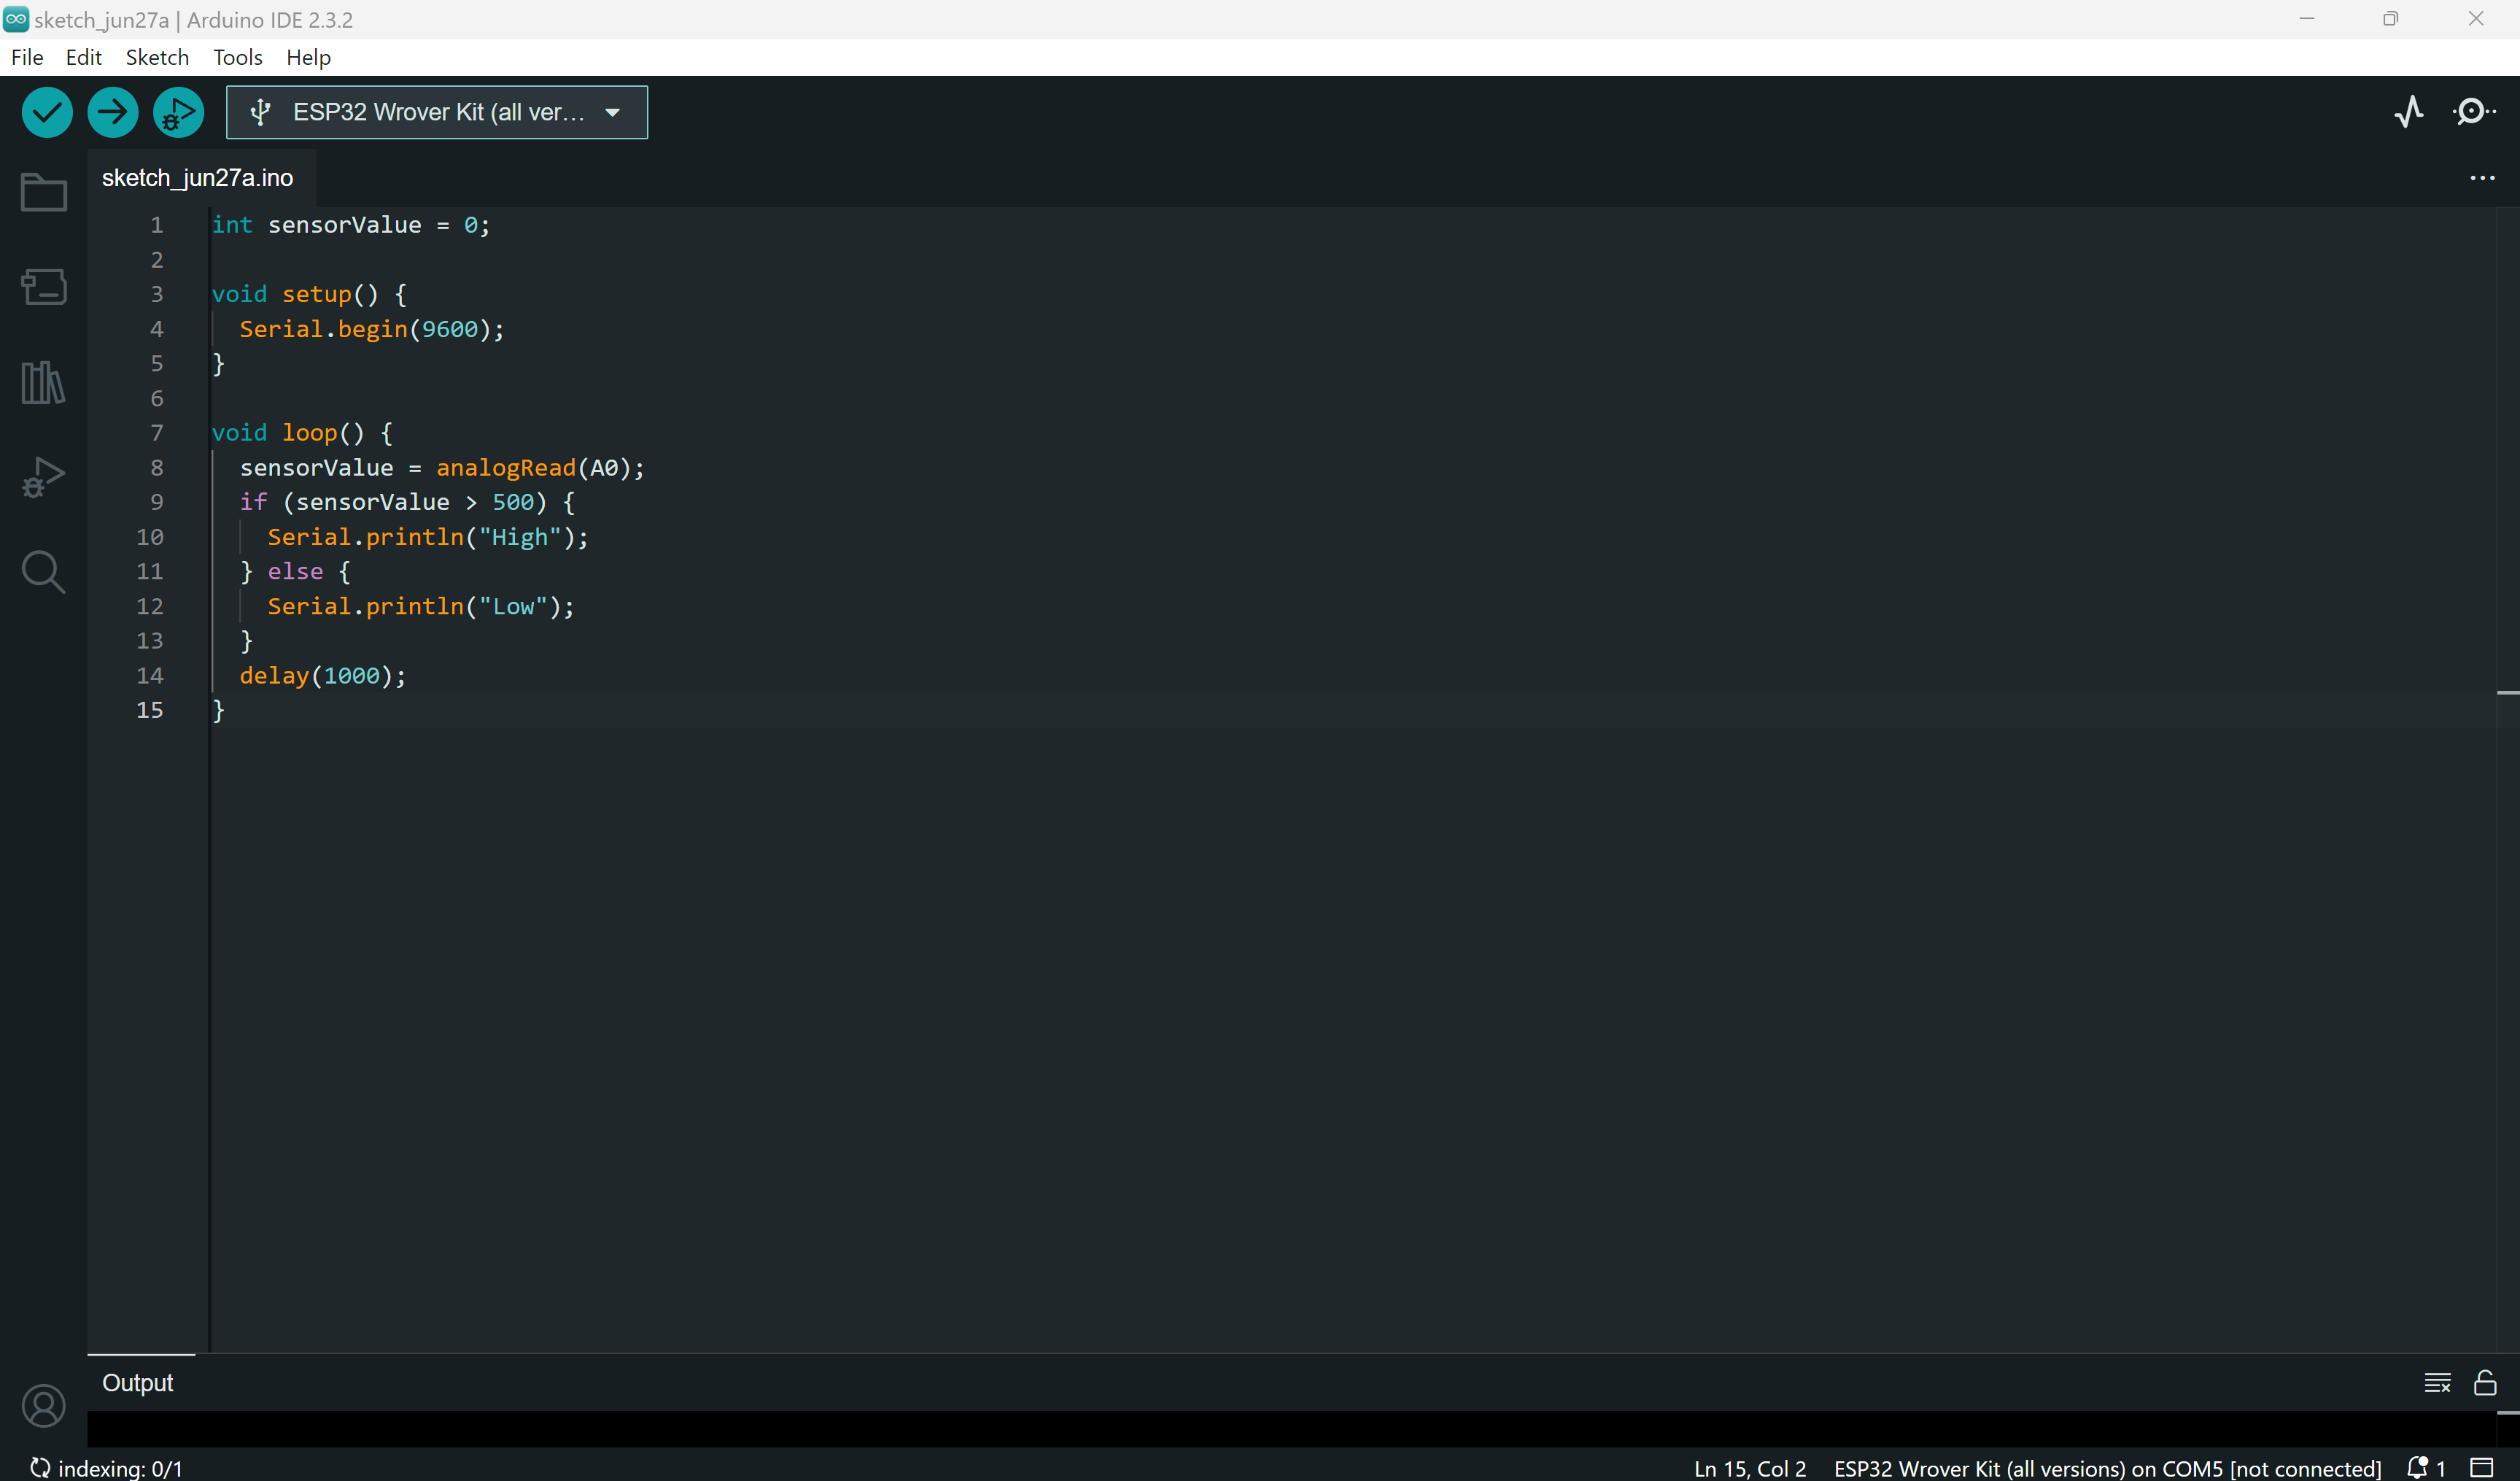
\includegraphics[width=\textwidth]{fig/fig8.png}
	\caption{C++ Conditions}
	\label{fig:8}
\end{figure}
\clearpage
\noindent\textbf{Eksempel: \texttt{case}}
\begin{lstlisting}[language=C++]
	int ledPin = 13;
	int command = 1;
	int button = 8;
	
	// Initialize with LOW because of pull-down resistor
	int lastButtonState = LOW;
	
	// Current reading from the input pin 
	int buttonState; 
	
	// the last time the output pin was toggled
	unsigned long lastDebounceTime = 0;
	
	// the debounce time; increase if the output flickers 
	unsigned long debounceDelay = 50; 
	
	void setup() {
		pinMode(ledPin, OUTPUT);
		pinMode(button, INPUT); 
		Serial.begin(9600);
		
		// Ensure LED is off initially
		digitalWrite(ledPin, LOW); 
	}
	
	void loop() {
		// Read the state of the switch into a local variable:
		int reading = digitalRead(button);
		
		// Check to see if you just pressed the button
		// (i.e. the input went from LOW to HIGH), and you've 
		//waited long enough
		// since the last press to ignore any noise:
		if (reading != lastButtonState) {
			// reset the debouncing timer
			lastDebounceTime = millis();
		}
		Serial.println(reading);
		if ((millis() - lastDebounceTime) > debounceDelay) {
			// whatever the reading is at, it's been there for 
			// longer than the debounce
			// delay, so take it as the actual current state:
			
			// if the button state has changed:
			if (reading != buttonState) {
				buttonState = reading;
				
				// only toggle the LED if the new button state is 
				//HIGH
				if (buttonState == HIGH) {
					switch (command) {
						case 1:
						Serial.println(buttonState);
						command = 0;
						break;
						case 0:
						Serial.println(buttonState);
						command = 1;
						break;
						default:
						// Do nothing
						break;
					}
				}
			}
		}
		
		// Save the reading. Next time through the loop, 
		// it'll be the lastButtonState:
		lastButtonState = reading;
		
		// Actions
		switch (command) {
			case 1:
			digitalWrite(ledPin, HIGH); // Turn LED on
			break;
			case 0:
			digitalWrite(ledPin, LOW); // Turn LED off
			break;
			default:
			// Do nothing
			break;
		}
	}
\end{lstlisting}
\clearpage
\section{C++ Loops}
\textbf{Teori:} Loops bruges til at udføre en blok kode gentagne gange. De mest almindelige loops er \texttt{while} og \texttt{for} loops. While loop udfører kodeblokken så længe betingelsen er sand, mens for loop bruges til at gentage en blok kode et bestemt antal gange. Loops er essentielle for gentagne opgaver som sensorlæsninger og LED blinkning.

\subsubsection{C++ While Loop}
\textbf{Teori:} \texttt{while} loop kontrollerer en betingelse og udfører kodeblokken gentagne gange så længe betingelsen er sand. Dette er nyttigt til opgaver, der skal fortsætte, indtil en bestemt tilstand ændres.
\newline\newline
\noindent\textbf{Eksempel:}
\begin{lstlisting}[language=C++]
	int i = 0;
	
	void setup() {
		Serial.begin(9600);
	}
	
	void loop() {
		while (i < 5) {
			Serial.println(i);
			i++;
		}
		delay(1000); // wait for a second before running again
	}
\end{lstlisting}
\begin{figure}[h!]
	\centering
	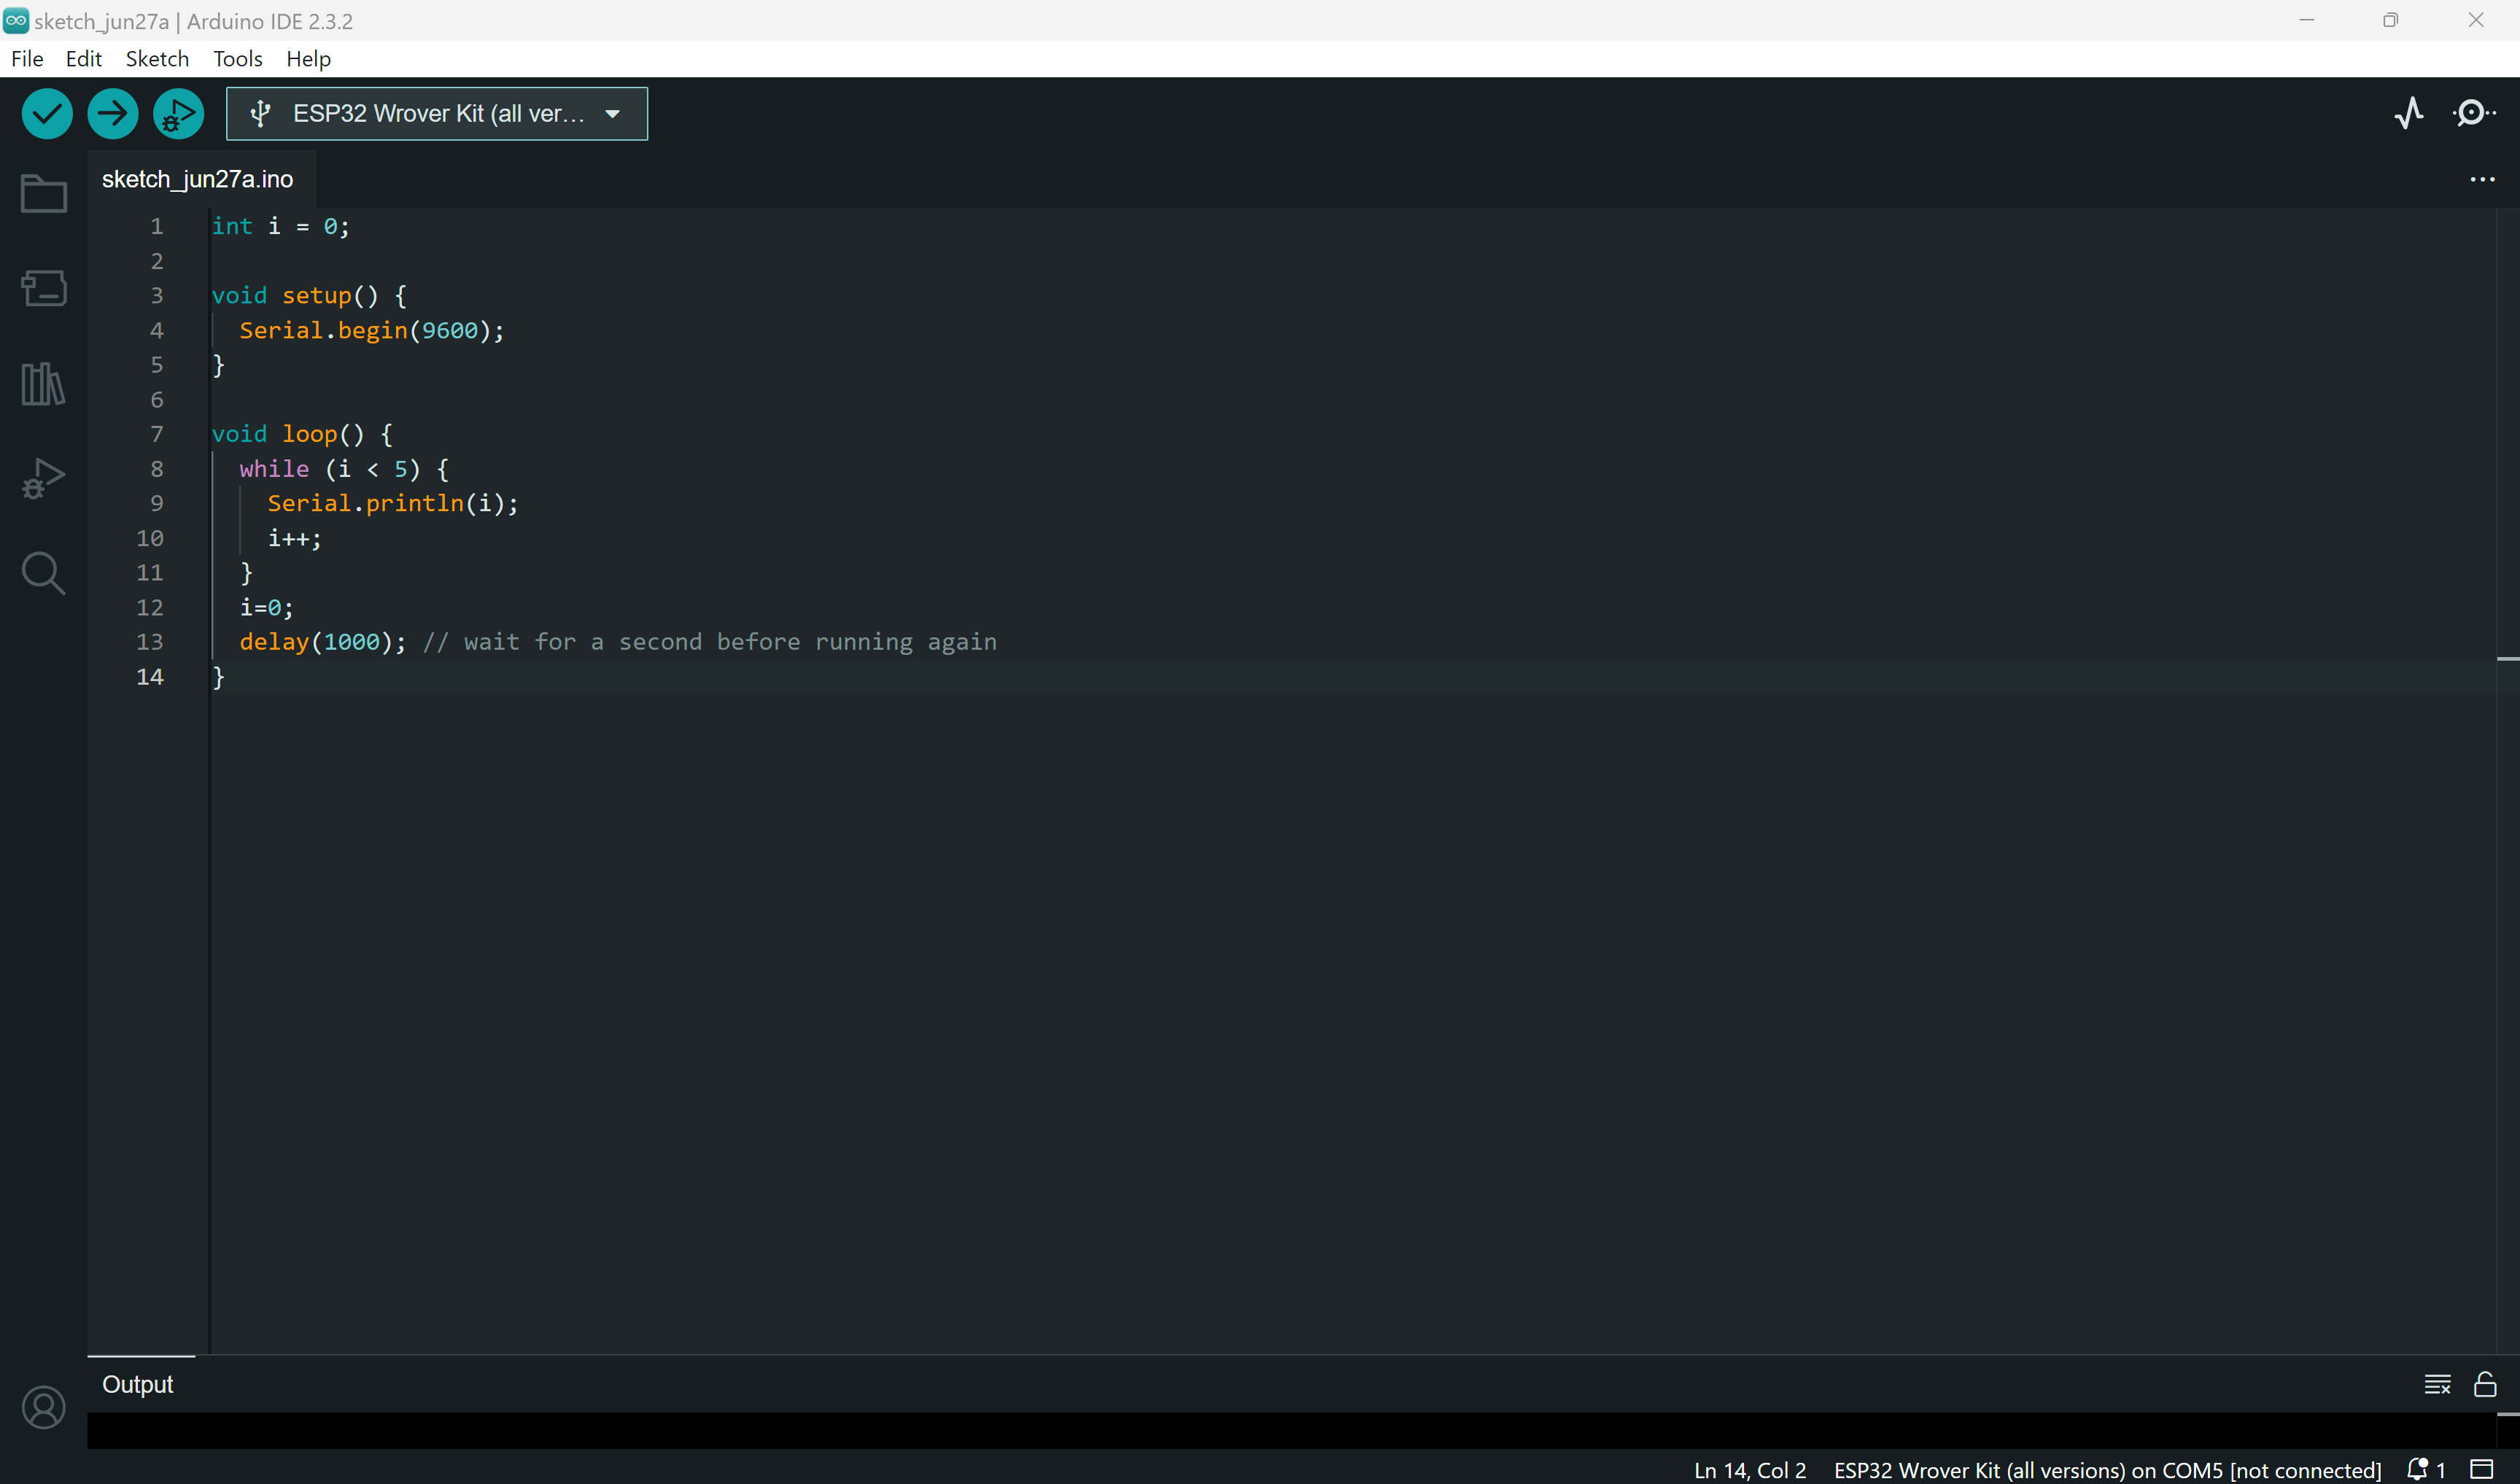
\includegraphics[width=\textwidth]{fig/fig9.png}
	\caption{while}
	\label{fig:9}
\end{figure}

\subsubsection{C++ For Loop}
\textbf{Teori:} \texttt{for} loop initialiserer en variabel, kontrollerer en betingelse og opdaterer variablen i hver iteration. For loops bruges ofte, når antallet af iterationer er kendt på forhånd.
\newline\newline
\noindent\textbf{Eksempel:}
\begin{lstlisting}[language=C++]
	void setup() {
		Serial.begin(9600);
	}
	
	void loop() {
		for (int i = 0; i < 5; i++) {
			Serial.println(i);
		}
		delay(1000); // wait for a second before running again
	}
\end{lstlisting}
\begin{figure}[h!]
	\centering
	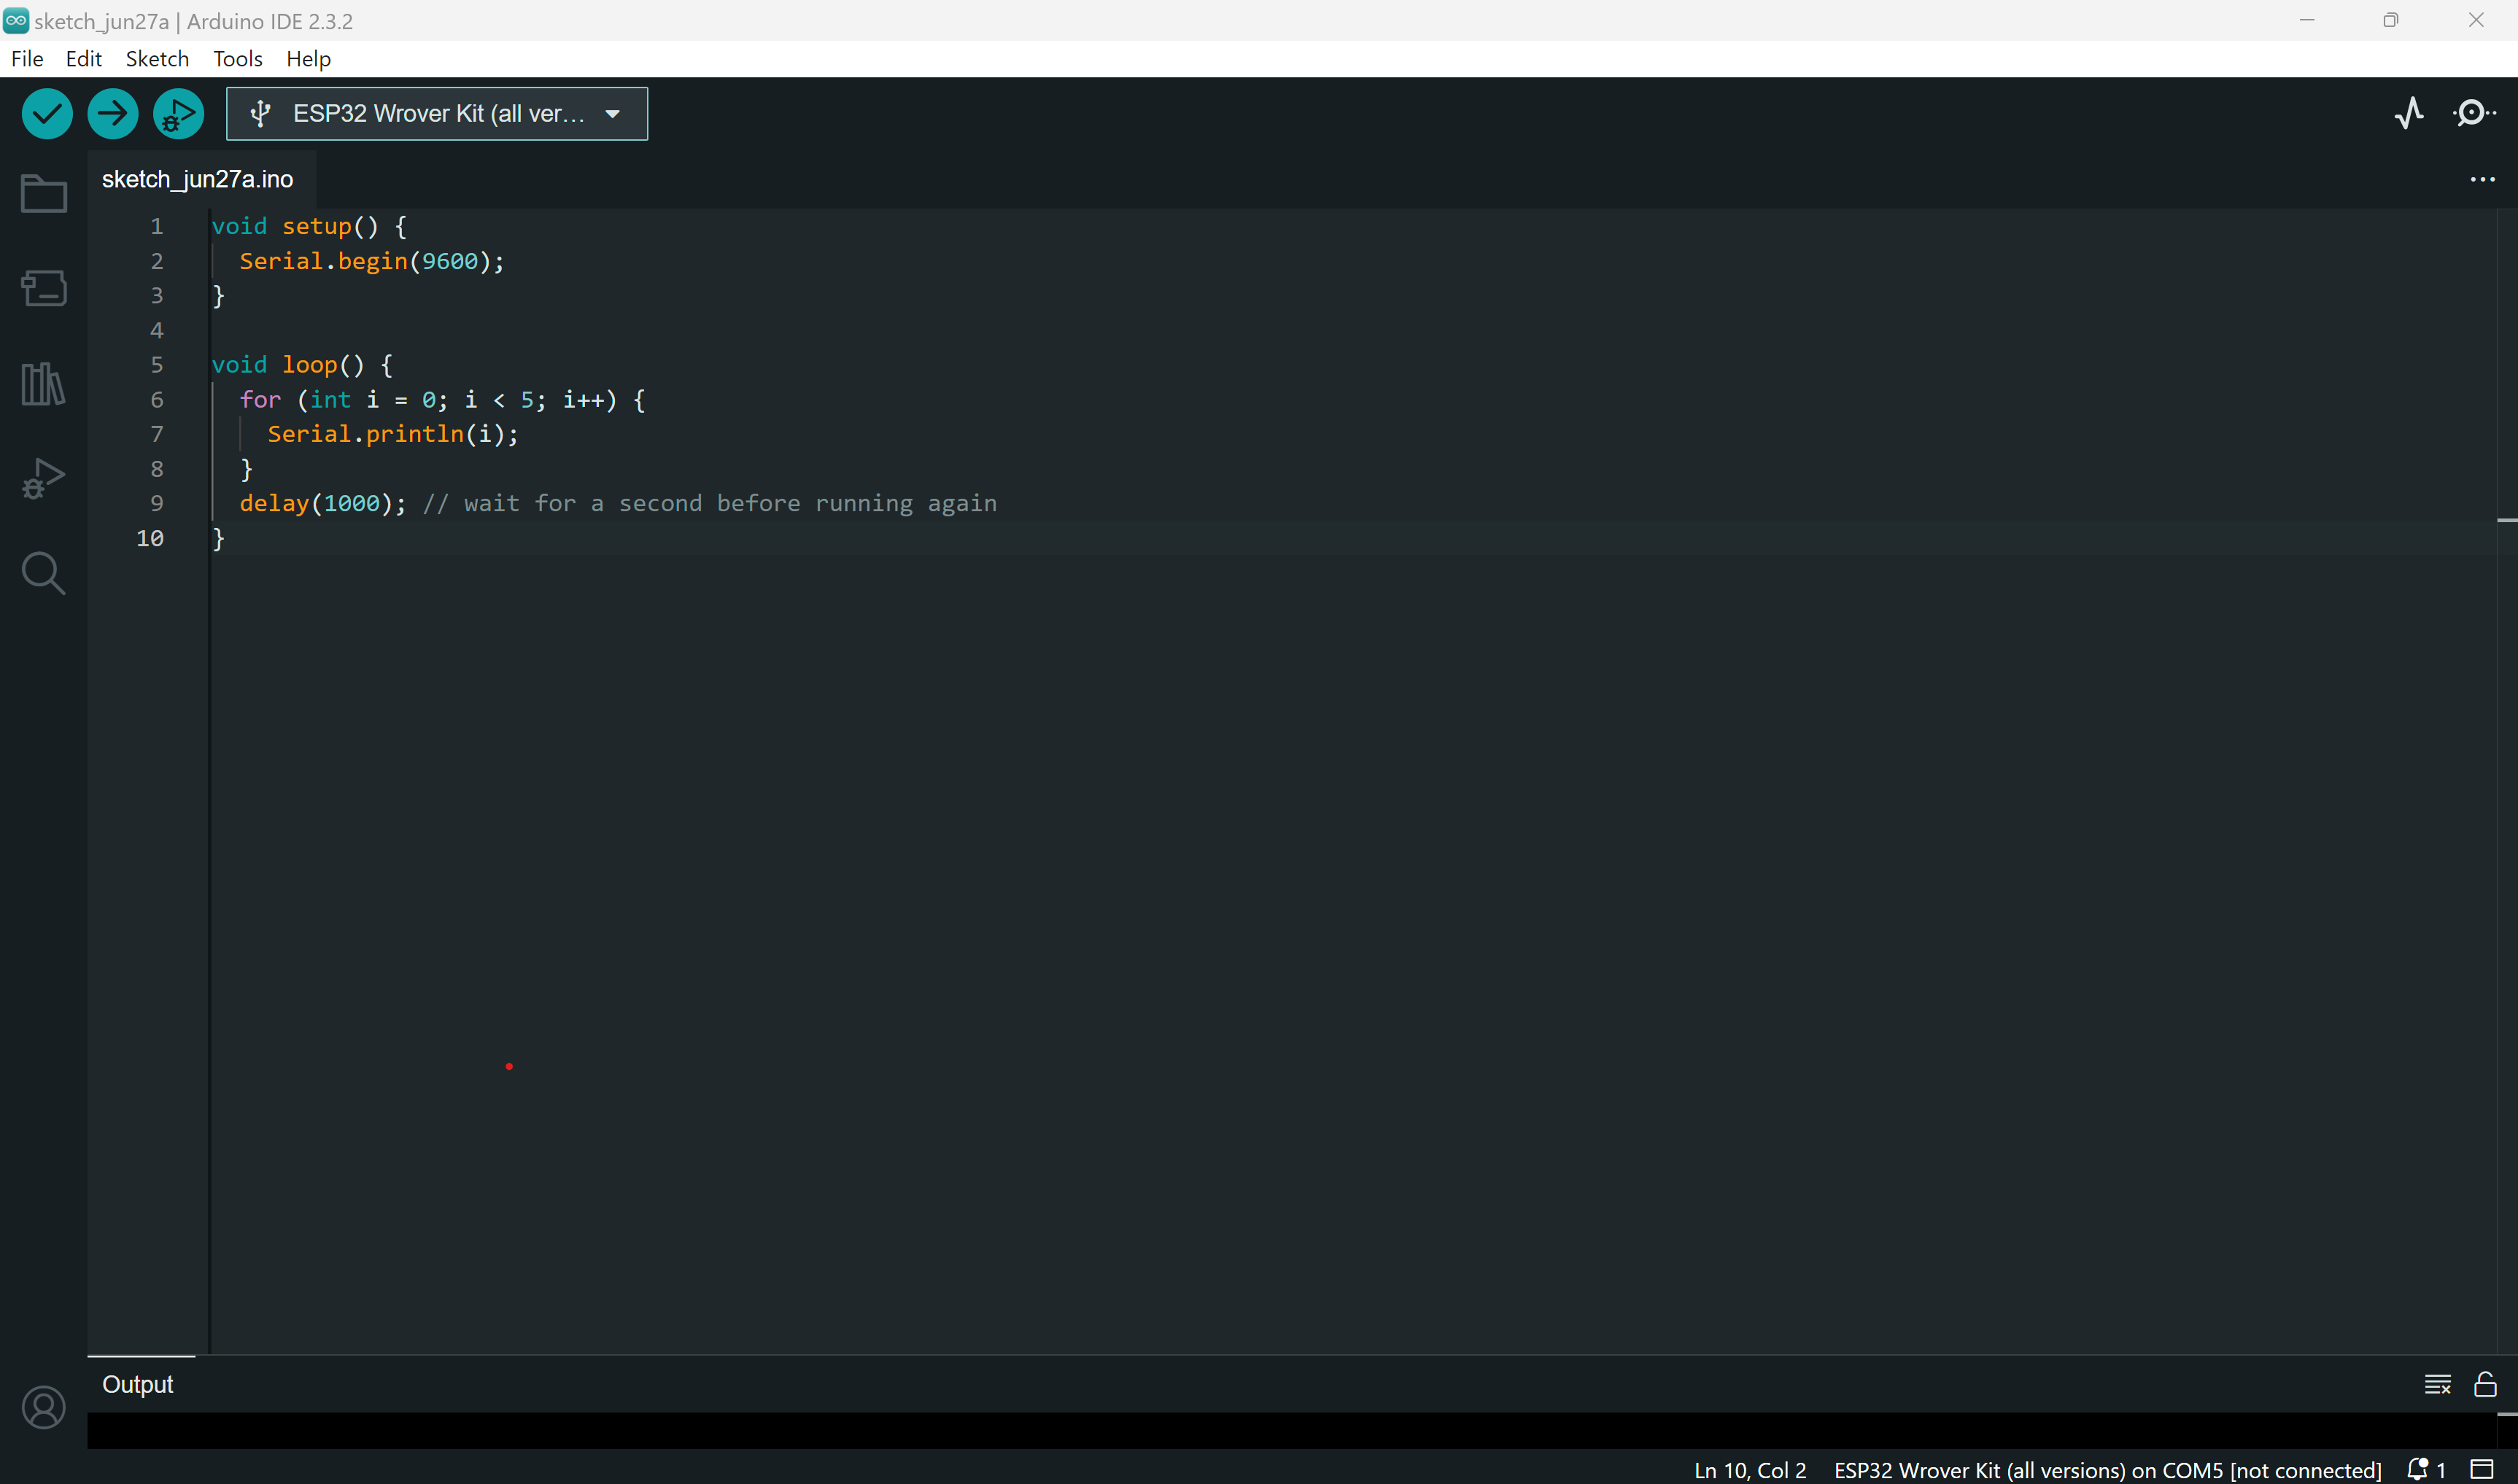
\includegraphics[width=\textwidth]{fig/fig10.png}
	\caption{For Loop}
	\label{fig:10}
\end{figure}

\section{C++ Functions}
\textbf{Formål:} Dette afsnit dækker funktioner i C++, herunder parameteroverførsel, overloading, scope og rekursion. Studerende vil lære at skrive og bruge funktioner til at strukturere og organisere deres kode på Arduino. Funktioner gør koden mere modulær og genanvendelig.

\textbf{Læringsmål:} Efter at have læst dette afsnit forventes det, at studerende kan:
\begin{itemize}
	\item Skrive og kalde funktioner i Arduino-kode.
	\item Forstå og anvende funktionsparametre i Arduino.
	\item Implementere funktion overloading hvor det er relevant.
	\item Forstå begrebet scope og livstid af variabler i Arduino-kode.
	\item Anvende rekursion i løsningen af problemer på Arduino.
\end{itemize}

\subsection{C++ Functions}
\textbf{Teori:} Funktioner er blokke af kode, der udfører en specifik opgave og kan genbruges flere steder i programmet. Funktioner kan tage parametre og returnere værdier. Dette gør det muligt at sende data til og modtage data fra funktioner.
\newline\newline
\noindent\textbf{Eksempel:}
\begin{lstlisting}[language=C++]
	void blink(int times) {
		for (int i = 0; i < times; i++) {
			digitalWrite(13, HIGH);
			delay(500);
			digitalWrite(13, LOW);
			delay(500);
		}
	}
	
	void setup() {
		pinMode(13, OUTPUT);
	}
	
	void loop() {
		blink(3); // call the blink function with parameter 3
		delay(1000); // wait for a second before running again
	}
\end{lstlisting}
\begin{figure}[h!]
	\centering
	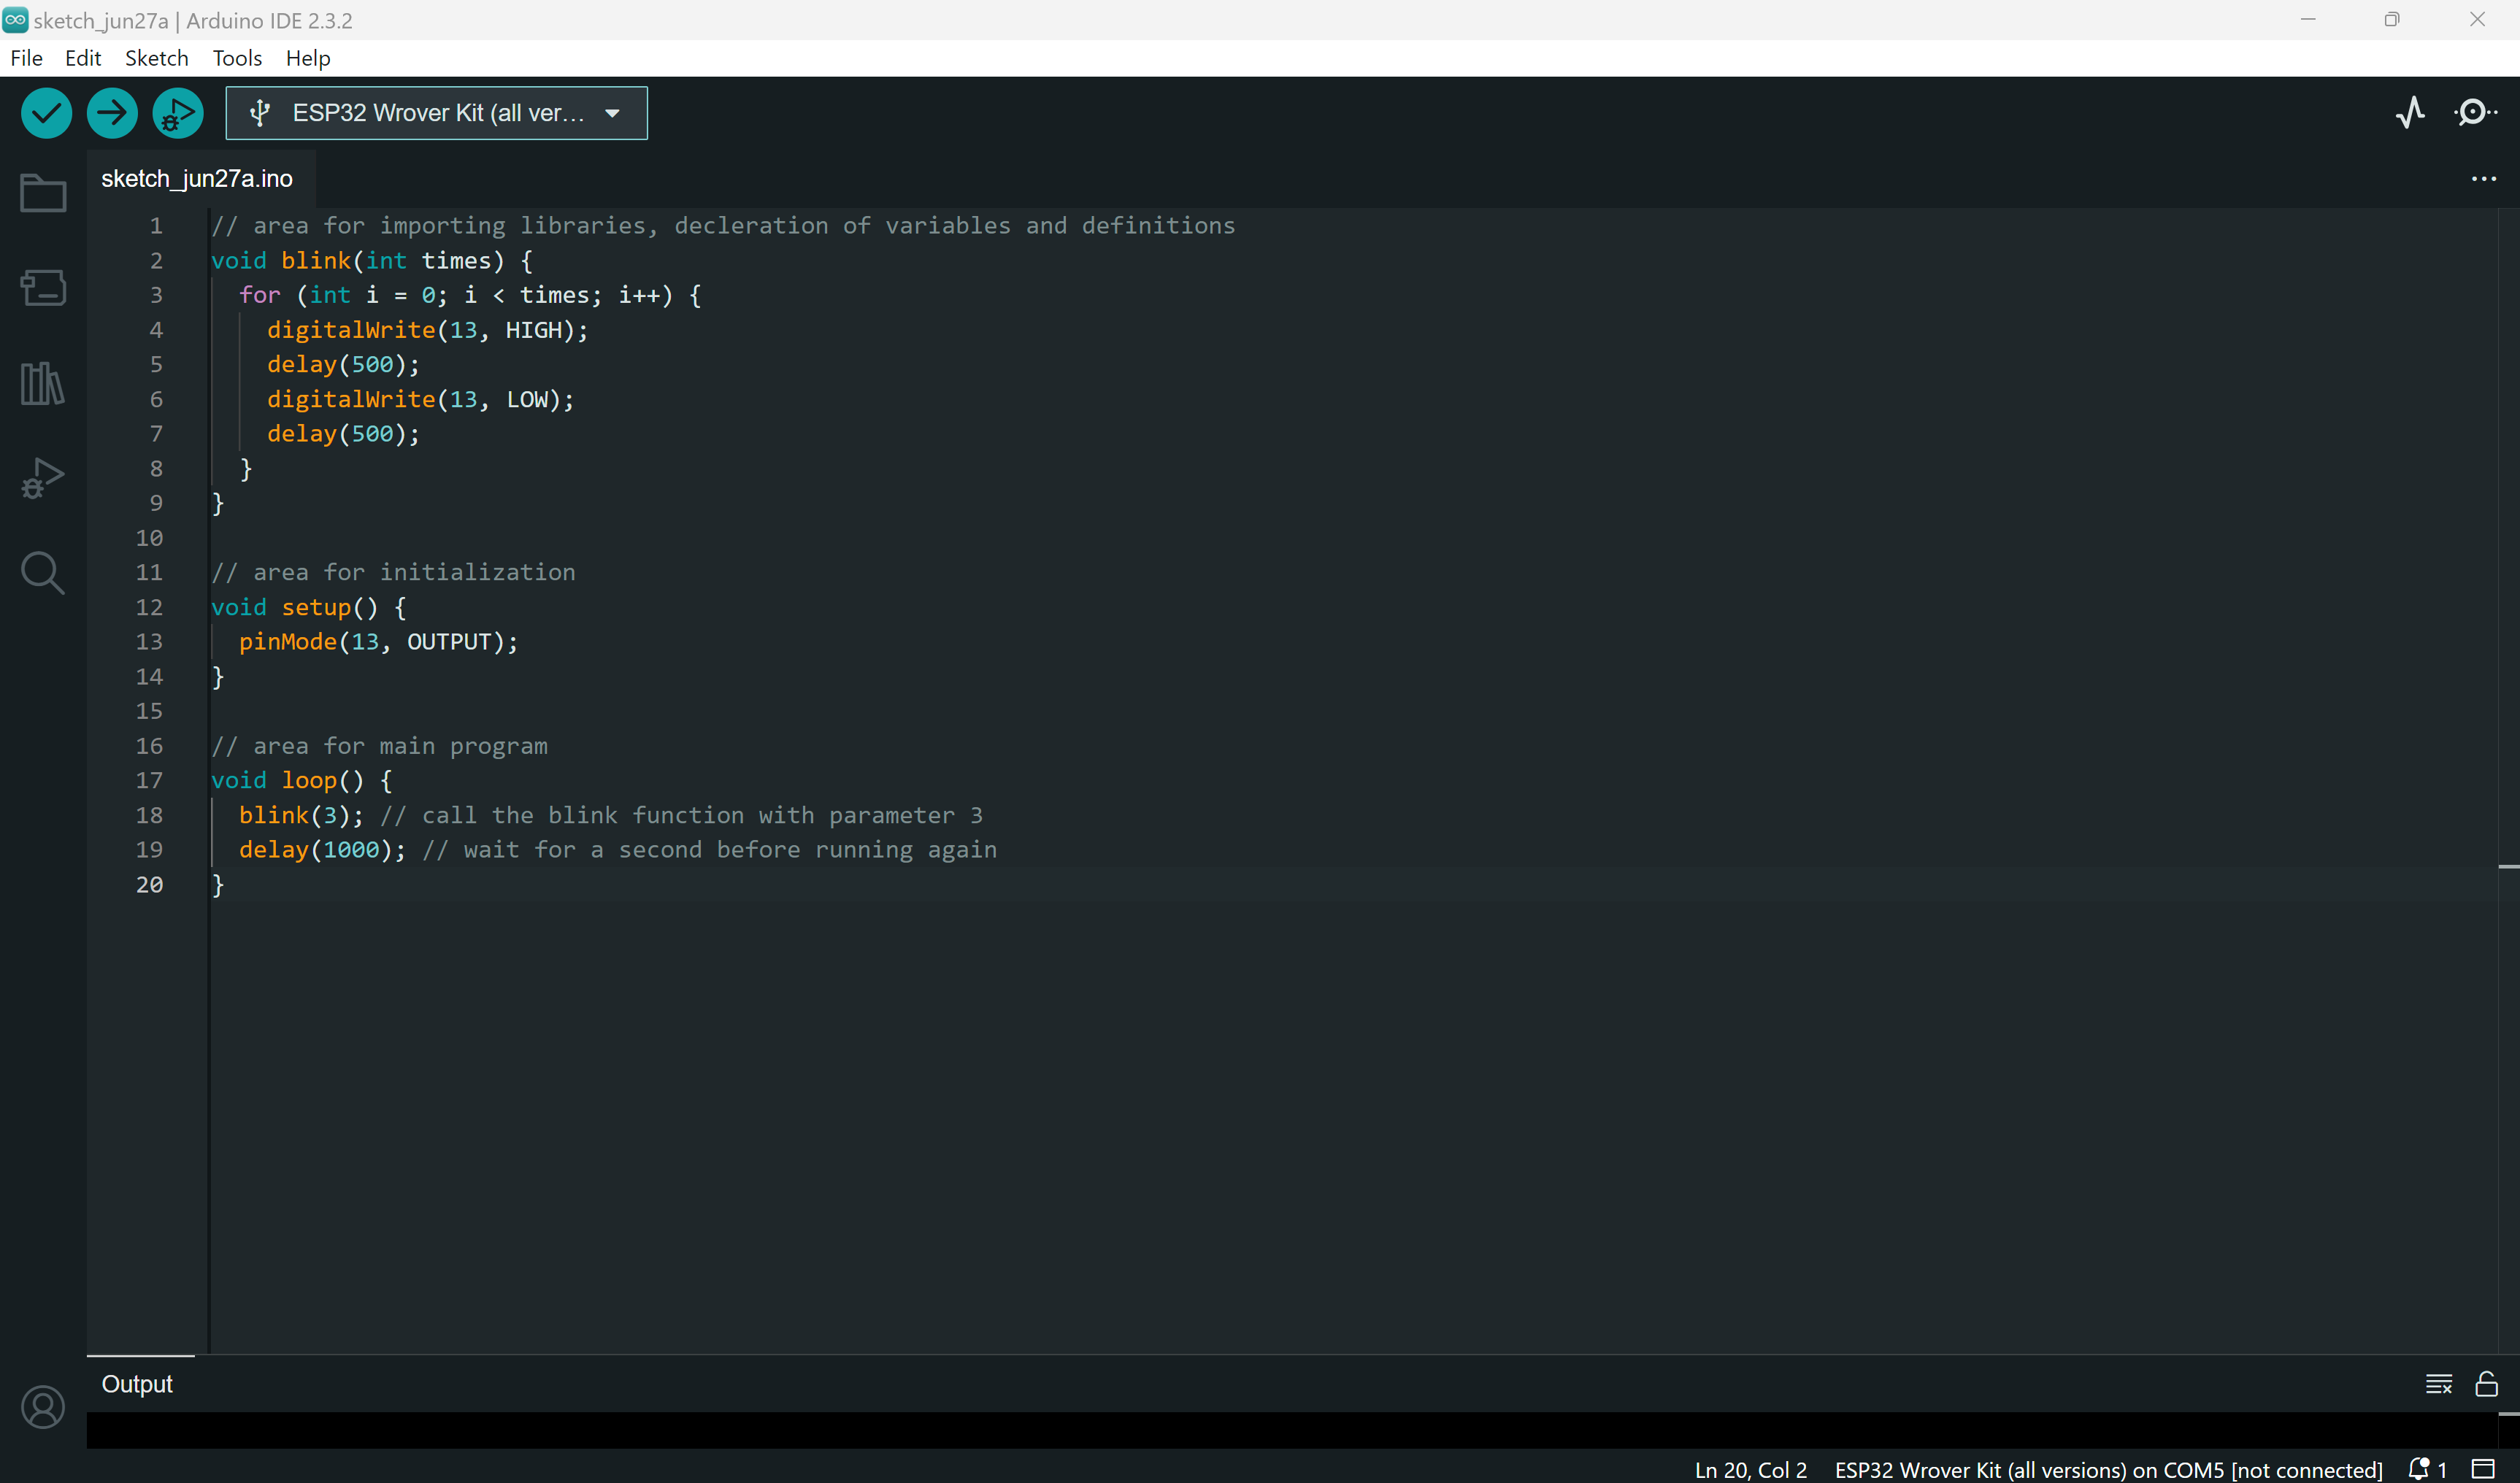
\includegraphics[width=\textwidth]{fig/fig11.png}
	\caption{text}
	\label{fig:11}
\end{figure}

\subsection{C++ Function Parameters}
\textbf{Teori:} Funktioner kan modtage input via parametre, som kan bruges inden i funktionen. Parametre specificeres i funktionsdeklarationen og defineres, når funktionen kaldes. Dette gør det muligt at skrive mere fleksible og genanvendelige funktioner.
\newline\newline
\noindent\textbf{Eksempel:}
\begin{lstlisting}[language=C++]
	void setup() {
		Serial.begin(9600);
	}
	
	void printMessage(String message) {
		Serial.println(message);
	}
	
	void loop() {
		printMessage("Hello, Arduino!"); // pass a string to the function
		delay(1000);
	}
\end{lstlisting}
\begin{figure}[h!]
	\centering
	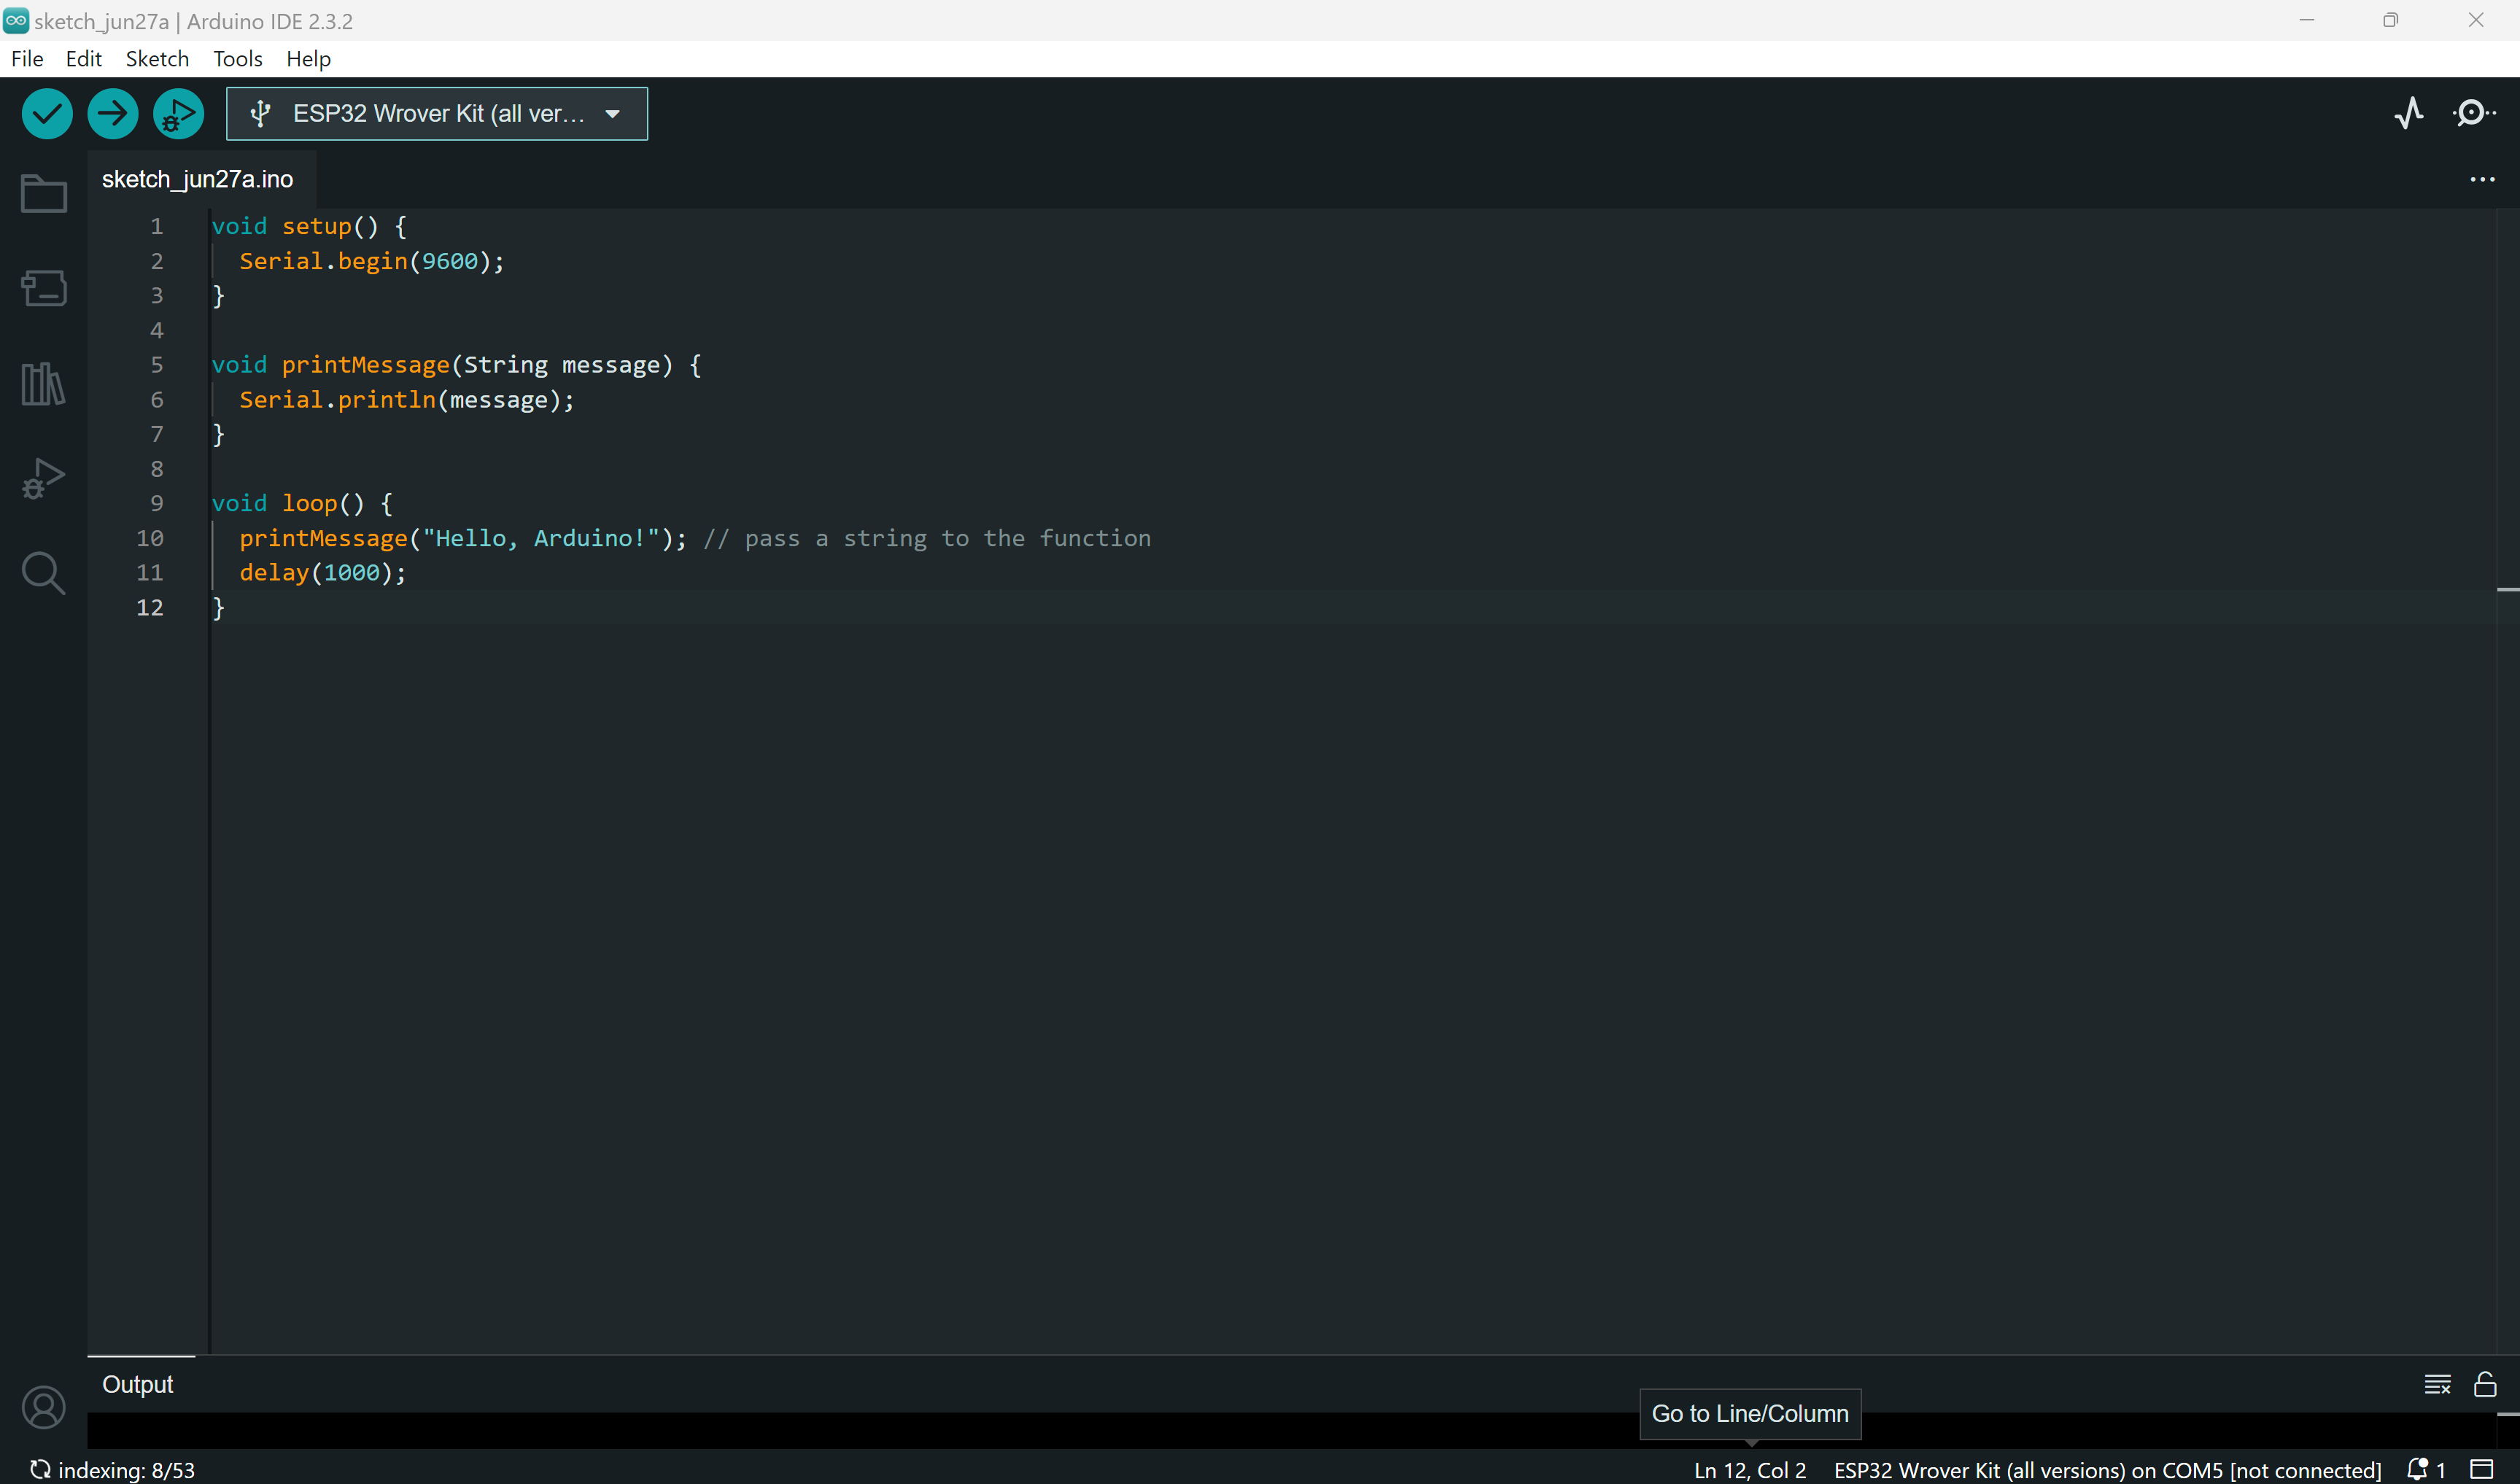
\includegraphics[width=\textwidth]{fig/fig12.png}
	\caption{C++ Function Parameters}
	\label{fig:12}
\end{figure}

\chapter{Arduino pins og special funktioner}
\section{pinMode i Arduino}
\textbf{pinMode()} funktionen i Arduino bruges til at konfigurere en specifik pin på mikrocontrolleren som enten en \textbf{input} eller \textbf{output}. Dette er et vigtigt skridt i opsætningen af hardware, da det bestemmer, hvordan en pin vil opføre sig under programkørslen. 
\newline\newline\noindent
Når en pin er konfigureret som \textbf{input}, kan den læse signaler fra sensorer eller knapper, hvilket betyder, at den kan modtage information fra omgivelserne. Når en pin er konfigureret som \textbf{output}, kan den sende signaler til komponenter som LED'er, motorer eller relæer, hvilket gør det muligt at styre disse enheder.

\begin{lstlisting}[language=C++, caption=Eksempel på brug af pinMode]
	void setup() {
		pinMode(13, OUTPUT);  // Sætter pin 13 som output (f.eks. til en LED)
		pinMode(7, INPUT);    // Sætter pin 7 som input (f.eks. til en knap)
	}
	
	void loop() {
		// Kode til at styre og læse fra pins
	}
\end{lstlisting}
I eksemplet ovenfor konfigureres pin 13 som en output, hvilket gør den velegnet til at tænde og slukke en LED. Pin 7 er konfigureret som input, hvilket gør den i stand til at læse signaler fra en knap. Dette er en grundlæggende, men afgørende funktion i Arduino-programmering, som giver brugeren kontrol over, hvordan mikrocontrolleren interagerer med eksterne komponenter.

\section{digitalRead og digitalWrite i Arduino}
\textbf{digitalRead()} og \textbf{digitalWrite()} er to essentielle funktioner i Arduino, der bruges til at læse og skrive digitale signaler på mikrocontrollerens pins.

\subsection{digitalRead()}
\textbf{digitalRead()} bruges til at læse statusen på en specificeret pin, som tidligere er sat op som \textbf{INPUT} med \texttt{pinMode()}. Denne funktion returnerer enten \texttt{HIGH} eller \texttt{LOW}, afhængigt af om der er spænding på pinnen (typisk 5V eller 3.3V for \texttt{HIGH}) eller ej (0V for \texttt{LOW}).
\begin{lstlisting}[language=C++, caption=Eksempel på brug af digitalRead]
	int buttonState = 0;
	
	void setup() {
		pinMode(7, INPUT);  // Sætter pin 7 som input
	}
	
	void loop() {
		buttonState = digitalRead(7);  // Læser tilstanden af pin 7
		if (buttonState == HIGH) {
			// Kode hvis knappen er trykket ned
		} else {
			// Kode hvis knappen ikke er trykket ned
		}
	}
\end{lstlisting}
I eksemplet ovenfor bruges \texttt{digitalRead()} til at afgøre, om en knap tilsluttet pin 7 er trykket ned (pinnen er \texttt{HIGH}) eller ej (\texttt{LOW}).

\subsection{digitalWrite()}
\textbf{digitalWrite()} bruges til at sætte en specifik pin til enten \texttt{HIGH} eller \texttt{LOW}. Dette gør det muligt at tænde eller slukke komponenter som LED'er, motorer eller relæer. For at bruge \texttt{digitalWrite()}, skal pinnen først være konfigureret som \textbf{OUTPUT} med \texttt{pinMode()}.

\begin{lstlisting}[language=C++, caption=Eksempel på brug af digitalWrite]
	void setup() {
		pinMode(13, OUTPUT);  // Sætter pin 13 som output
	}
	
	void loop() {
		digitalWrite(13, HIGH);   // Tænder LED tilsluttet pin 13
		delay(1000);              // Venter i 1 sekund
		digitalWrite(13, LOW);    // Slukker LED
		delay(1000);              // Venter i 1 sekund
	}
\end{lstlisting}
I eksemplet ovenfor bruges \texttt{digitalWrite()} til at tænde og slukke en LED tilsluttet pin 13. Funktionen skifter mellem \texttt{HIGH} (tænder LED'en) og \texttt{LOW} (slukker LED'en), med en forsinkelse på 1 sekund mellem hver skift.
\newline\newline\noindent
\textbf{digitalRead()} og \textbf{digitalWrite()} er grundlæggende byggesten i Arduino-programmering, da de giver kontrol over, hvordan mikrocontrolleren interagerer med digitale indgange og udgange.

\section{analogRead og analogWrite i Arduino}
\textbf{analogRead()} og \textbf{analogWrite()} er to funktioner i Arduino, der bruges til at læse og skrive analoge signaler på mikrocontrollerens pins.

\subsection{analogRead()}
\textbf{analogRead()} bruges til at læse værdien fra en analog indgangspin. Arduinoen har flere analoge indgange (typisk mærket som \texttt{A0}, \texttt{A1}, osv.), der kan læse spændinger mellem 0 og 5V (eller 0 og 3.3V afhængigt af modellen). Denne funktion returnerer en værdi mellem 0 og 1023, hvor 0 svarer til 0V og 1023 svarer til maksimal spænding.
\begin{lstlisting}[language=C++, caption=Eksempel på brug af analogRead]
	int sensorValue = 0;
	
	void setup() {
		Serial.begin(9600);  // Initialiserer seriel kommunikation
	}
	
	void loop() {
		sensorValue = analogRead(A0);  // Læser værdien fra pin A0
		Serial.println(sensorValue);   // Udskriver værdien til seriel monitor
		delay(500);                    // Venter i 0,5 sekunder
	}
\end{lstlisting}
I eksemplet ovenfor bruges \texttt{analogRead()} til at læse en spænding fra en sensor tilsluttet pin \texttt{A0}. Værdien udskrives derefter til seriel monitoren.

\subsection{analogWrite()}
\textbf{analogWrite()} bruges til at generere en pulsbreddemoduleret (PWM) signal på en specifik pin. Arduinoen har flere PWM-udgange (typisk markeret med en tilde, f.eks. \texttt{~3}, \texttt{~5}, osv.). Funktionen \texttt{analogWrite()} tager en værdi mellem 0 og 255, hvor 0 betyder ingen output (0V) og 255 betyder maksimal output (5V eller 3.3V, afhængigt af modellen).

\begin{lstlisting}[language=C++, caption=Eksempel på brug af analogWrite]
	int brightness = 0;
	
	void setup() {
		pinMode(9, OUTPUT);  // Sætter pin 9 som output
	}
	
	void loop() {
		for (brightness = 0; brightness <= 255; brightness++) {
			analogWrite(9, brightness);  // Justerer lysstyrken på LED'en
			delay(10);                   // Venter i 10 ms
		}
		for (brightness = 255; brightness >= 0; brightness--) {
			analogWrite(9, brightness);  // Justerer lysstyrken på LED'en
			delay(10);                   // Venter i 10 ms
		}
	}
\end{lstlisting}
I eksemplet ovenfor bruges \texttt{analogWrite()} til at kontrollere lysstyrken på en LED tilsluttet pin 9. Værdien varieres fra 0 (slukket) til 255 (maksimal lysstyrke) i en glidende overgang.
\newline\newline\noindent
\textbf{analogRead()} og \textbf{analogWrite()} er vigtige funktioner i Arduino-programmering, da de giver mulighed for at interagere med analoge signaler og justere output i forhold til en kontinuerlig skala.

\section{delay og millis i Arduino}
\textbf{delay()} og \textbf{millis()} er to funktioner i Arduino, der bruges til at arbejde med tid og timing i programmer.

\subsection{delay()}
\textbf{delay()} er en funktion, der forsinker udførelsen af programmet i et bestemt antal millisekunder. Funktionen stopper al kodeudførelse i det angivne tidsrum, hvilket kan være nyttigt, når du ønsker at skabe en simpel pause eller forsinkelse mellem handlinger.

\begin{lstlisting}[language=C++, caption=Eksempel på brug af delay]
	void setup() {
		pinMode(13, OUTPUT);  // Sætter pin 13 som output
	}
	
	void loop() {
		digitalWrite(13, HIGH);  // Tænder LED'en tilsluttet pin 13
		delay(1000);             // Venter i 1000 ms (1 sekund)
		digitalWrite(13, LOW);   // Slukker LED'en
		delay(1000);             // Venter i 1000 ms (1 sekund)
	}
\end{lstlisting}
I eksemplet ovenfor bruges \texttt{delay()} til at skabe en 1-sekunds pause, hvor en LED tændes og slukkes skiftevis. Det er en enkel måde at styre tid i dit program på, men det blokerer programudførelsen, hvilket betyder, at ingen anden kode kan køre, mens \texttt{delay()} udføres.

\subsection{millis()}
\textbf{millis()} er en funktion, der returnerer antallet af millisekunder, der er gået, siden Arduinoen startede. Funktionen bruges ofte til at udføre tidstagning uden at blokere programudførelsen, hvilket gør den ideel til opgaver, der kræver nøjagtig timing uden at stoppe al anden kodeudførelse.
\begin{lstlisting}[language=C++, caption=Eksempel på brug af millis]
	unsigned long previousMillis = 0;
	const long interval = 1000;  // Intervallet er sat til 1000 ms (1 sekund)
	
	void setup() {
		pinMode(13, OUTPUT);  // Sætter pin 13 som output
	}
	
	void loop() {
		unsigned long currentMillis = millis();
		
		if (currentMillis - previousMillis >= interval) {
			previousMillis = currentMillis;  // Opdaterer tidligere tid
			digitalWrite(13, !digitalRead(13));  // Skifter LED'ens tilstand
		}
	}
\end{lstlisting}
I eksemplet ovenfor bruges \texttt{millis()} til at blinke en LED uden at blokere programudførelsen. LED'en skifter tilstand (tændt/slukket) hver gang intervallet på 1 sekund er gået. Fordelen ved \texttt{millis()} er, at det tillader andre funktioner i \texttt{loop()} at køre samtidigt, hvilket er vigtigt i komplekse programmer, hvor flere opgaver skal udføres parallelt.
\newline\newline\noindent
\textbf{delay()} er enkel og nem at bruge, men den stopper programmet midlertidigt, hvilket kan være uønsket i mere avancerede applikationer. \textbf{millis()} giver en mere fleksibel måde at håndtere tid og timing på uden at stoppe andre dele af programmet, hvilket gør det til et foretrukket valg i mange tilfælde.


